\lab{Introduction to Wavelets}{Intro to Wavelets}
\objective{In the context of Fourier analysis, one seeks to represent a function as a sum of sinusoids.
A drawback to this approach is that the Fourier transform only captures global frequency information, and local information is lost; we can know which frequencies are the most prevalent, but not when or where they occur.
The Wavelet transform provides an alternative approach that avoids this shortcoming and is often a superior analysis technique for many types of signals and images.
}

\section*{The Discrete Wavelet Transform} % ===================================

In wavelet analysis, we seek to analyze a function by considering its \emph{wavelet decomposition}.
The wavelet decomposition of a function is a way of expressing the function as a linear combination
of a particular family of basis functions.
In this way, we can represent a function by the sequence of coefficients (called
\emph{wavelet coefficients}) defining this linear combination.
The mapping from a function to its sequence of wavelet coefficients is called the \emph{discrete
wavelet transform}.

This situation is entirely analogous to the discrete Fourier transform. Instead of using trigonometric functions
as our basis, we use a different family
of basis functions. In Wavelet analysis, we determine the family of basis functions by first starting
off with a function $\psi$ called the \emph{wavelet} and a function $\phi$ called the \emph{scaling function}
(these functions are also called the mother and father wavelets, respectively). We then generate
countably many basis functions (sometimes called baby wavelets) from these two functions:
\begin{align*}
\psi_{m,k}(x) &= \psi(2^mx - k)\\
\phi_{m,k}(x) &= \phi(2^mx - k),
\end{align*}
where $m,k \in \mathbb{Z}$.
The historically first, and most basic, wavelet is called the \emph{Haar Wavelet},
given by
\[
\psi(x) =
 \begin{cases}
  1 & \text{if } 0 \leq x < \frac{1}{2} \\
  -1 & \text{if } \frac{1}{2} \leq x < 1 \\
  0 & \text{otherwise.}
 \end{cases}
\]
% It might be nice to plot this function and include the image in the lab.
The associated scaling function is given by
\[
\phi(x) =
 \begin{cases}
 1 & \text{if } 0 \leq x < 1 \\
 0 & \text{otherwise.}
 \end{cases}
\]

In the case of finitely-sampled signals and images, only finitely many wavelet coefficients are nonzero.
Depending on the application, we are often only interested in the coefficients corresponding to a subset of the basis functions.
Since a given family of wavelets forms an orthogonal set, we can compute the wavelet coefficients
by taking inner products (i.e. by integrating). This direct approach is not particularly efficient,
however. Just as there are fast algorithms for computing the fourier transform (e.g. the FFT),
we can efficiently calculate wavelet coefficients using techniques from signal processing.
In particular, we will use an \emph{iterative filterbank} to compute the transform.
% mathematical derivation?

Let's launch into an implementation of the one-dimensional discrete wavelet transform.
The key operations in the algorithm are the discrete convolution ($*$) and down-sampling ($DS$).
The inputs to the algorithm are a one-dimensional array $X$ (the signal that we want to transform), a one-dimensional
array $L$ (called the \emph{low-pass filter}), a one-dimensional array $H$ (the \emph{high-pass filter}), and a positive
integer $n$ (controlling to what degree we wish to transform the signal, i.e. how many wavelet coefficients we wish to compute).
The low-pass and high-pass filters can be derived from the wavelet and scaling function.
The low-pass filter extracts low frequency information, which gives us an approximation of the signal.
This approximation highlights the overall (slower-moving) pattern
without paying too much attention to the high frequency details, which to the eye (or ear) may be unhelpful noise.
However, we also need to extract the high-frequency details with the high-pass filter. While they may sometimes be
nothing more than unhelpful noise, there are applications where they are the most important part of the signal; for example,
details are very important if we are sharpening a blurry image or increasing contrast.

For the Haar Wavelet, our filters are given by
\begin{align*}
L &= \begin{bmatrix}\frac{1}{\sqrt{2}} & \frac{1}{\sqrt{2}}\end{bmatrix}\\
H &= \begin{bmatrix}-\frac{1}{\sqrt{2}} & \frac{1}{\sqrt{2}}\end{bmatrix}.
\end{align*}
See Algorithm \ref{alg:1d_wavelet} and Figure \ref{fig:filterbank} for the specifications.
\begin{algorithm}
\begin{algorithmic}[1]
\Procedure{dwt}{$X, L, H, n$}
	\State $i \gets 0$						\Comment{Some initialization steps}
    \State $A_i \gets X$
    \While{$i < n$}
        \State $D_{i+1} \gets \,\,DS(A_i * H)$ \Comment{High-pass filtering}
        \State $A_{i+1} \gets \,\,DS(A_i * L)$ \Comment{Low-pass filtering}
        \State $i \gets i + 1$
    \EndWhile
    \State \pseudoli{return} $A_n,D_n, D_{n-1},\ldots, D_1$.
\EndProcedure
\end{algorithmic}
\caption{The one-dimensional discrete wavelet transform.}
\label{alg:1d_wavelet}
\end{algorithm}
\begin{figure}[H]
\centering
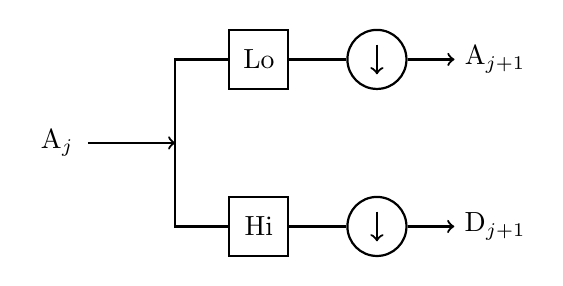
\begin{tikzpicture}[auto, node distance=1.5cm, thick, main node/.style={circle, draw}, LoHi/.style={rectangle, draw}, minimum size=.75cm]
    \node[draw=none](Aj){A$_j$};
    \node[draw=none](j1)[right of=Aj]{};
    \node[LoHi](Lo)[above right of=j1]{Lo};
    \node[LoHi](Hi)[below right of=j1]{Hi};
    \node[main node](1)[right of=Lo]{};
    \node[main node](2)[right of=Hi]{};
    \node[draw=none](Aj+1)[right of=1]{A$_{j+1}$};
    \node[draw=none](Dj+1)[right of=2]{D$_{j+1}$};

\foreach \s/\t in {Aj/j1.center, 1/Aj+1, 2/Dj+1}{
    \draw[->] (\s) -- (\t);}
\foreach \s/\t in {j1.center/Lo, j1.center/Hi}{
    \draw[](\s) |- (\t);}
\foreach \s/\t in {Lo/1, Hi/2}{
    \draw[](\s) -- (\t);}
\foreach \s in {1, 2}{
    \draw[->, shorten >=.2cm, shorten <=.2cm] (\s.north) -- (\s.south);}
\end{tikzpicture}

\vspace{1cm}

\begin{center}
\begin{tikzpicture}
% Key
    \node[draw=none, node distance=2.5cm](K)[below of=Aj]{Key:};
    \node[rectangle, draw, minimum size=.5cm, node distance=1cm](rect)[right of=K]{};
    \node[draw=none, node distance=1.3cm](conv)[right of=rect]{= convolve};
    \node[circle, draw, minimum size=.5cm, node distance=1cm](circ)[below of=rect]{};
    \node[draw=none, node distance=1.5cm](conv)[right of=circ]{= downsample};
    \draw[->, shorten >=.1cm, shorten <=.1cm] (circ.north) -- (circ.south);
\end{tikzpicture}
\end{center}
\caption{The one-dimensional discrete wavelet transform
implemented as a filter bank.}
\label{fig:filterbank}
\end{figure}
At each stage of the algorithm, we filter the signal into an approximation and its details.
Note that the algorithm returns a sequence of one dimensional arrays
\[A_n, D_n, D_{n-1}, \ldots, D_1.\]
If the input signal $X$ has length $2^m$ for
some $m \geq n$ and we are using the Haar wavelet, then $A_n$ has length $2^{m-n}$, and $D_i$ has length $2^{m-i}$
for $i=1,\ldots,n$. The arrays $D_i$ are outputs of the high-pass filter, and thus represent high-frequency
details.
Hence, these arrays are known as \emph{details}.
The array $A_n$ is computed by recursively passing the signal through the low-pass filter, and hence it
represents the low-frequency structure in the signal.
In fact, $A_n$ can be seen as a smoothed approximation of the original signal, and is called the \emph{approximation}.

As noted earlier, the key mathematical operations are convolution and down-sampling.
To accomplish the convolution, we simply use a function in SciPy.
\begin{lstlisting}
>>> import numpy as np
>>> from scipy.signal import fftconvolve
>>> # initialize the filters
>>> L = np.ones(2)/np.sqrt(2)
>>> H = np.array([-1,1])/np.sqrt(2)
>>> # initialize a signal X
>>> X = np.sin(np.linspace(0,2*np.pi,16))
>>> # convolve X with L
>>> fftconvolve(X,L)
[ -1.84945741e-16   2.87606238e-01   8.13088984e-01   1.19798126e+00
   1.37573169e+00   1.31560561e+00   1.02799937e+00   5.62642704e-01
   7.87132986e-16  -5.62642704e-01  -1.02799937e+00  -1.31560561e+00
  -1.37573169e+00  -1.19798126e+00  -8.13088984e-01  -2.87606238e-01
  -1.84945741e-16]
\end{lstlisting}
The convolution operation alone gives us redundant information, so we down-sample to keep only what we need.
In particular, we will down-sample by a factor
of two, which means keeping only every other entry:
\begin{lstlisting}
>>> # down-sample an array X
>>> sampled = X[1::2]
\end{lstlisting}
Putting these two operations together, we can obtain the approximation coefficients in one
line of code:
\begin{lstlisting}
>>> A = fft.convolve(X,L)[1::2]
\end{lstlisting}
Computing the detail coefficients is done in exactly the same way, replacing $L$ with $H$.
\begin{problem}
Write a function that calculates the discrete wavelet transform as described above.
The output should be a list of one-dimensional NumPy arrays in the
following form: $[A_n, D_n, \ldots, D_1]$.

The main body of your function should be a loop in which you calculate two arrays: the $i$-th approximation
and detail coefficients. Append the detail coefficients array to your list, and feed the approximation array
back into the loop. When the loop is finished, append the approximation array. Finally, reverse the order of your list
to adhere to the required return format.

Test your function by calculating the Haar wavelet coefficients of a noisy sine signal for $n=4$:

\begin{lstlisting}
>>> domain = np.linspace(0,4*np.pi, 1024)
>>> noise =  np.random.randn(1024)*.1
>>> noisysin = np.sin(domain) + noise
>>> coeffs = dwt(noisysin, L, H, 4)
\end{lstlisting}

Plot your results and verify that they match the plots in Figure \ref{fig:dwt1D}.
\end{problem}

We can now transform a one-dimensional signal into its wavelet coefficients,
but the reverse transformation is just as important.
Luckily, we can reconstruct a signal from the approximation and detail coefficients.
We reverse the effects of the filterbank, using slightly modified filters, essentially adding the details back into the
signal at each stage until we reach the original.
The Haar wavelet filters for the inverse transformation are
\begin{align*}
L &= \begin{bmatrix}\frac{1}{\sqrt{2}} & \frac{1}{\sqrt{2}}\end{bmatrix}\\
H &= \begin{bmatrix}\frac{1}{\sqrt{2}} & -\frac{1}{\sqrt{2}}\end{bmatrix}.
\end{align*}

Suppose we have the wavelet coefficients $A_n$ and $D_n$. Consulting Figure \ref{fig:filterbank},
we can recreate $A_{n-1}$ by tracing the schematic backwards: $A_n$ and $D_n$ are first
\emph{up-sampled}, then they are convolved with $L$ and $H$, respectively, and finally
added together to obtain $A_{n-1}$. Up-sampling means doubling the length of an array
by inserting a 0 at every other position.

\newpage

\begin{lstlisting}
>>> # up-sample the coefficient arrays A, D
>>> up_A = np.zeros(2*A.size)
>>> up_A[::2] = A
>>> up_D = np.zeros(2*D.size)
>>> up_D[::2] = D
>>> # now convolve and add, but discard last entry
>>> A = fftconvolve(up_A,L)[:-1] + fftconvolve(up_D,H)[:-1]
\end{lstlisting}

Now that we have $A_{n-1}$, we repeat the process with $A_{n-1}$ and $D_{n-1}$ to obtain
$A_{n-2}$. Proceed for a total of $n$ steps (one for each $D_n, D_{n-1},\ldots ,D_1$) until we have obtained $A_0$.
Since $A_0$ is defined to be the original
signal, we have finished the inverse transformation.
% TODO: proof that this works, perhaps in an appendix...

\begin{problem} % Inverse wavelet transform
Write a function that calculates the inverse wavelet transform as described above.
The inputs should be a list of arrays (of the same form as the output of your discrete
wavelet transform function), the low-pass filter, and the high-pass filter.
The output should be a single array, the recovered signal.

Note that the input list of arrays has length $n+1$ (consisting of $A_n$ together with
$D_n, D_{n-1}, \ldots, D_1$), so your code should perform the process given above $n$ times.

In order to check your work, compute
the discrete wavelet transform of a random array for different values of $n$, then compute the inverse
transform.
Compare the original signal with the recovered signal using \li{np.allclose}.
\end{problem}

\section*{The PyWavelets Module} % ============================================

Having implemented our own version of the basic 1-dimensional wavelet transform, we now turn to
PyWavelets, a Python library for Wavelet Analysis.
It provides convenient and efficient methods to calculate the one- and two-dimensional discrete Wavelet
transform, as well as much more.

If you have the Anaconda distribution, then you can install PyWavelets simply with the command:

\begin{lstlisting}
$ conda install -c ioos pywavelets=0.4.0
\end{lstlisting}

Once the package has been installed on your machine, type the following to get started:

\begin{lstlisting}
>>> import pywt
\end{lstlisting}

Performing the discrete Wavelet transform is very simple.
Below, we compute the one-dimensional transform for a sinusoidal signal.

\begin{lstlisting}
>>> import numpy as np
>>> f = np.sin(np.linspace(0,8*np.pi, 256)) # build the sine wave
>>> fw = pywt.wavedec(f, 'haar') # compute the wavelet coefficients of f
\end{lstlisting}

The variable \li{fw} is now a list of arrays, starting with the final approximation
frame, followed by the various levels of detail coefficients, just like the output
of the wavelet transform function that you already coded.
Plot the level 2 detail and verify that it resembles a blocky sinusoid.

\begin{lstlisting}
>>> from matplotlib import pyplot as plt
>>> plt.plot(fw[-2], linestyle='steps')
>>> plt.show()
\end{lstlisting}

To reconstruct the signal, we simply call the function \li{waverec}:

\begin{lstlisting}
>>> f_prime = pywt.waverec(fw, 'haar') # reconstruct the signal
>>> np.allclose(f_prime, f) # compare with the original
True
\end{lstlisting}

The second positional argument, as you will notice, is a string that gives the name of the wavelet to be used.
We first used the Haar wavelet, with which you are already familiar.
PyWavelets supports a number of different Wavelets, however, which you can list by executing the following code:

\begin{lstlisting}
>>> # list the available Wavelet families
>>> print pywt.families()
['haar', 'db', 'sym', 'coif', 'bior', 'rbio', 'dmey']
>>> # list the available wavelets in the coif family
>>> print pywt.wavelist('coif')
['coif1', 'coif2', 'coif3', 'coif4', 'coif5']

\end{lstlisting}
Different wavelets have different properties; the most suitable wavelet is dependent on the specific application.
See Figure \ref{fig:more_wavelets} for the plots of a couple of additional wavelets.
\begin{figure}[H]
\begin{subfigure}[b]{0.45\textwidth}
    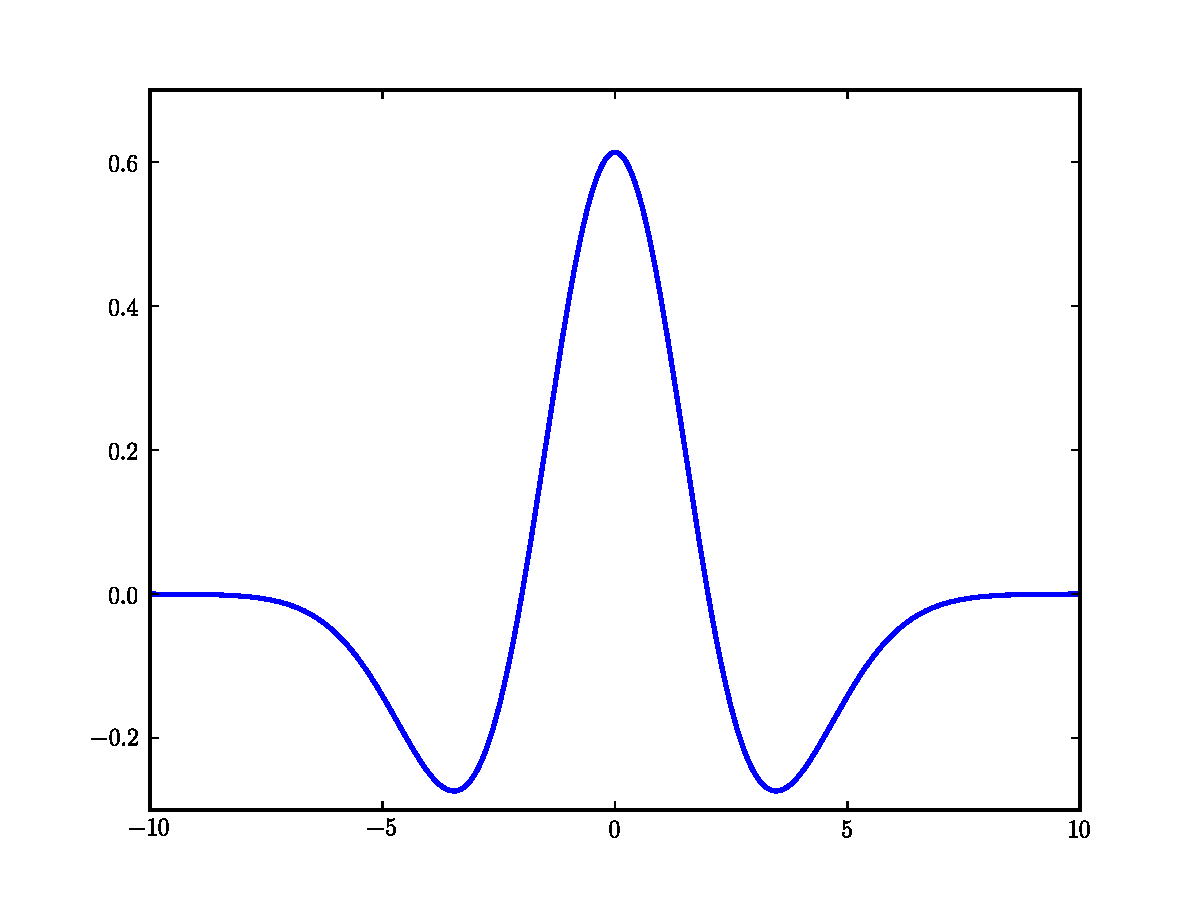
\includegraphics[width=\textwidth]{mexicanHat}
\end{subfigure}
\begin{subfigure}[b]{0.45\textwidth}
    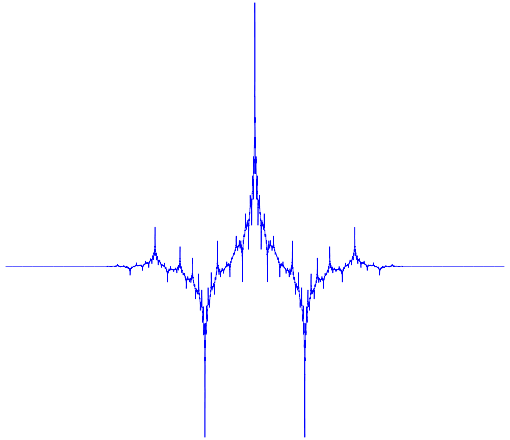
\includegraphics[width=\textwidth]{db5_3}
\end{subfigure}
\caption{Examples of different mother wavelets.}
\label{fig:more_wavelets}
\end{figure}

\section*{The 2-dimensional Wavelet Transform} % ==============================

We can generalize the wavelet transform for two dimensions much as we generalized the fourier transform.
This allows us to perform wavelet analysis on, for example, digital images.
In particular, we can calculate the wavelet transform of a two-dimensional
array  by first transforming the rows, and then the columns of the array.

When implemented as an iterative filterbank, each pass through the filterbank yields an approximation plus three sets of detail coefficients
rather than just one.
More specifically, if the two-dimensional array $X$ is the input to the filterbank, we obtain arrays $LL$, $LH$, $HL$, and $HH$,
where $LL$ is a smoothed approximation of $X$ and the other three arrays contain wavelet coefficients capturing high-frequency
oscillations in vertical, horizontal, and diagonal directions.
In the jargon of signal processing, the arrays $LL$, $LH$, $HL$, and $HH$ are called \emph{subbands}.
By recursively feeding any or all of the subbands back into the filterbank, we can decompose an input array into a collection
of many subbands.
This decomposition can be represented schematically by a dyadic partition of a rectangle, called a \emph{subband pattern}.
The subband pattern for one pass of the filterbank is shown in Figure \ref{fig:2dsubbands}, with a concrete example given in Figure \ref{fig:dwt2D}.
\begin{figure}
\begin{tikzpicture}
%\node[draw, thick, minimum size=4cm](-2,-2) square (2,2) []{$A_k$};
\draw[thick] (-2,-2) rectangle (2,2);
\draw[step=2cm,thick,draw](4,-2) grid (8,2);
\draw[thick] (4,-2) -- (8,-2);

\node[draw=none]()at(0,0){$X$};
\node[draw=none]()at(5,1){$LL$};
\node[draw=none]()at(7,1){$LH$};
\node[draw=none]()at(5,-1){$HL$};
\node[draw=none]()at(7,-1){$HH$};
\draw[->, >=stealth', thick, shorten <=.2cm, shorten >=.2cm]
	(2,0)--(4,0);
\end{tikzpicture}
\caption{The subband pattern for one step in the 2-dimensional wavelet transform.}
\label{fig:2dsubbands}
\end{figure}
\begin{figure}
% the Mandrill image used to compute these images is found at http://homepages.cae.wisc.edu/~ece533/images/ (baboon.png)
\centering
        \begin{subfigure}{0.4\textwidth}\centering
                    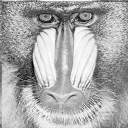
\includegraphics[width=\linewidth]{mandrill1.png}
       \end{subfigure}%
%    \hfill
        \begin{subfigure}{0.4\textwidth}\centering
                    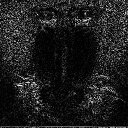
\includegraphics[width=\linewidth]{mandrill2.png}
       \end{subfigure}%
    \hfill
        \begin{subfigure}{0.4\textwidth}\centering
                    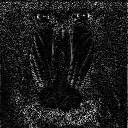
\includegraphics[width=\linewidth]{mandrill3.png}
       \end{subfigure}%
 %   \hfill
        \begin{subfigure}{0.4\textwidth}\centering
                    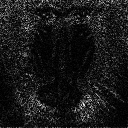
\includegraphics[width=\linewidth]{mandrill4.png}
       \end{subfigure}
    \caption{Subbands for the Mandrill image after one pass through the filterbank.
    Note how the upper left subband ($LL$) is an approximation of the original Mandrill image, while the other
    three subbands highlight the stark vertical, horizontal, and diagonal changes in the image.\\
    Original image source: \url{http://sipi.usc.edu/database/}.}
    \label{fig:dwt2D}
\end{figure}
The wavelet coefficients that we obtain from a two-dimensional wavelet transform are very useful in a variety of image processing tasks.
They allow us to analyze and manipulate images in terms of both their
frequency and spatial properties, and at differing levels of resolution.
Furthermore, wavelet bases often have the remarkable ability to represent
images in a very \textit{sparse} manner -- that is, most of the image
information is captured by a small subset of the wavelet coefficients.
This is the key fact for wavelet-based image compression.

PyWavelets provides a simple way to calculate the subbands resulting from one pass through the filterbank.
\begin{lstlisting}
>>> from scipy.misc import imread
>>> fingerprint = imread(filename, True)  # flag True produces a grayscale image
>>> # use the db4 wavelet with periodic extension
>>> lw = pywt.dwt2(fingerprint, 'db4', mode='per')
\end{lstlisting}
Note that the \li{mode} keyword argument determines the type of extension mode (required for the convolution
operation).
The variable \li{lw} is a list. The first entry of the list is the $LL$, or approximation, subband.
The second entry of the list is a tuple containing the remaining subbands, $LH$, $HL$, and $HH$ (in that order).
Plot these subbands as follows:
\begin{lstlisting}
>>> plt.subplot(221)
>>> plt.imshow(np.abs(lw[0]), cmap=plt.cm.Greys_r, interpolation='none')
>>> plt.subplot(222)
>>> plt.imshow(np.abs(lw[1][0]), cmap=plt.cm.Greys_r, interpolation='none')
>>> plt.subplot(223)
>>> plt.imshow(np.abs(lw[1][1]), cmap=plt.cm.Greys_r, interpolation='none')
>>> plt.subplot(224)
>>> plt.imshow(np.abs(lw[1][2]), cmap=plt.cm.Greys_r, interpolation='none')
>>> plt.show()
\end{lstlisting}

\begin{problem}
Plot the subbands of the file \li{swan_lake_polluted.png} as described above.
Compare this with the subbands the mandrill image shown in Figure \ref{fig:dwt2D}.
\end{problem}

\section*{Image Processing}
We are now ready to use the two-dimensional wavelet transform for image processing.
Wavelets are especially good at filtering out high-frequency noise from an image.
Just as we were able to pinpoint the noise added to the sin wave in Figure \ref{fig:dwt1D}, the majority of the noise added to an image will be contained in the final $LH$, $HL$, and $HH$ detail subbands of our wavelet decomposition.
If we decompose our image and reconstruct it with all subbands except these final subbands, we will eliminate most of the troublesome noise while preserving the primary aspects of the image.

We perform this cleaning as follows:
\begin{lstlisting}
image = imread(filename,True)
wavelet = pywt.Wavelet('haar')
WaveletCoeffs = pywt.wavedec2(image,wavelet)
new_image = pywt.waverec2(WaveletCoeffs[:-1], wavelet)
\end{lstlisting}

\begin{problem}
Write a function called \li{clean_image()} which accepts the name of a grayscale image file, and cleans high-frequency noise out of the image.
Load the image as an ndarray, and perform a wavelet decomposition using PyWavelets.
Reconstruct the image using all subbands except the last set of detail coefficients, and return this cleaned image as an ndarray.
\end{problem}

\newpage

\section*{Additional Material}

\subsection*{Image Compression} % ---------------------------------------------

Numerous image compression techniques have been developed over the years to reduce the cost of storing large quantities of images.
Transform methods based on Fourier and Wavelet analysis have long played an important role in these techniques; for example, the popular JPEG image compression standard is based on the discrete cosine transform.
The JPEG2000 compression standard and the FBI Fingerprint Image database, along with other systems, take the wavelet approach.

The general framework for compression is fairly straightforward.
First, the image to be compressed undergoes some form of preprocessing,
depending on the particular application.
Next, the discrete wavelet transform is used to calculate the wavelet coefficients, and these are then \textit{quantized}, i.e. mapped to a set of discrete values (for example, rounding to the nearest integer).
The quantized coefficients are then passed through an entropy encoder (such as Huffman Encoding), which reduces the number of bits required to store the coefficients.
What remains is a compact stream of bits that can then be saved or transmitted much more efficiently than the original image.
The steps above are nearly all invertible (the only exception being rounding), allowing us to almost perfectly reconstruct the image from the compressed bitstream.
See Figure \ref{tikz:wsqscheme}.

\begin{figure}[H]
\centering
\begin{tikzpicture}[rect/.style= {draw=none, node distance = 3cm},
	rect2/.style = {draw, thick, minimum width=3cm, minimum
	height=1cm}, >=stealth', shorten >=2pt]

\node[rect] (IM) [] {Image};
\node[rect2, node distance=3cm] (PR) [right of = IM]
	{Pre-Processing};
\node[rect2, node distance=4.5cm] (WD)[right of= PR]
	{Wavelet Decomposition};
\node[rect2, node distance=1.75cm](Q) [below=of PR.west, anchor=west]
	{Quantization};
\node[rect2, node distance = 1.75cm](EC)[below=of WD.west, anchor=west]
	{Entropy Coding};
\node[rect, node distance= 3.5cm](BS)[right of=EC]
	{Bit Stream};

\foreach \s/\t in {IM/PR, PR/WD, Q/EC, EC/BS}
	{\path[->, thick](\s) edge (\t);}
\draw[|-,-|,->, thick](WD.south) |-+(0,-1em)-| (Q.north);


\end{tikzpicture}
\caption{Wavelet Image Compression Schematic}
\label{tikz:wsqscheme}
\end{figure}

\begin{comment}

\subsection*{WSQ: The FBI Fingerprint Image Compression Algorithm} % ----------

The Wavelet Scalar Quantization (WSQ) algorithm is among the first successful wavelet-based image compression algorithms.
It solves the problem of storing millions of fingerprint scans efficiently while meeting the law enforcement requirements for high image quality.
This algorithm is capable of achieving compression ratios in excess of 10-to-1 while retaining excellent image quality;
see Figure \ref{fig:finger_compression}.
We will implement a basic version of this algorithm by writing a Python class that performs both the compression and decompression.
\begin{problem}
Begin your implementation by defining the class \li{WSQ} and adding an initialization method and the \li{compress}
method, as follows:
\begin{lstlisting}
class WSQ:
    """
    Perform compression using the Wavelet Scalar Quantization algorithm.
    All class attributes are set to None in __init__, but their values
    are initialized in the compress method.

    Attributes
    ----------
    _pixels : int, number of pixels in source image
    _s : float, scale parameter for image preprocessing
    _m : float, shift parameter for image preprocessing
    _Q : numpy array, quantization parameters q for each subband
    _Z : numpy array, quantization parameters z for each subband
    _bitstrings : list of 3 BitArrays, giving bit encodings for each group.
    _tvals : tuple of 3 lists of bools, indicating which subbands in each
             groups were encoded
    _shapes : tuple of 3 lists of tuples, giving shapes of each subband in each group
    _huff_maps : list of 3 dicts, mapping huffman index to bit pattern
    """
    def __init__(self):
        self._pixels = None
        self._s = None
        self._m = None
        self._Q = None
        self._Z = None
        self._bitstrings = None
        self._tvals = None
        self._shapes= None
        self._huff_maps = None

    def compress(self, img, r, gamma=2.5):
        """
        The main compression routine. It computes and stores bitstring representation
        of compressed image, along with other values needed for decompression.

        Parameters
        ----------
        img : numpy array containing 8-bit integer pixel values
        r : float, the closer to zero, the higher compression ratio
        gamma : float, a parameter used in quantization
        """
        pass
\end{lstlisting}

As we go through each step of the compression process throughout the remainder of the lab,
you will be adding methods and attributes to the class as directed.
You will also be implementing the \li{compress} method along the way.
As a first step in the \li{compress} method, calculate the number of pixels
in the input image, and store this number in the class attribute \li{_pixels}.
\end{problem}

\begin{figure}
\centering
\begin{subfigure}{.32\textwidth}
  \centering
  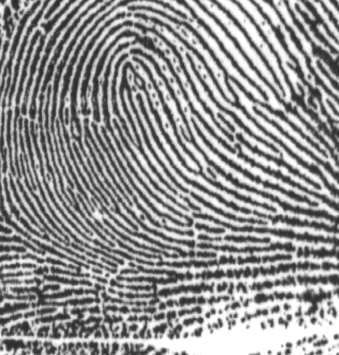
\includegraphics[width=.7\linewidth]{uncompressed_finger.png}
  \caption{Uncompressed}
  \label{fig:sub1}
\end{subfigure}%
\begin{subfigure}{.32\textwidth}
  \centering
  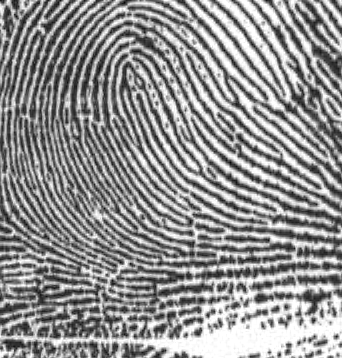
\includegraphics[width=.7\linewidth]{compressed_finger(30comp).png}
  \caption{12:1 compressed}
  \label{fig:sub1}
\end{subfigure}%
\begin{subfigure}{.32\textwidth}
  \centering
  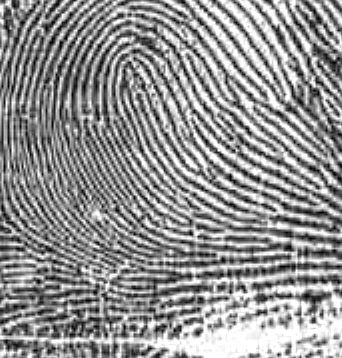
\includegraphics[width=.7\linewidth]{compressed_finger(60comp).png}
  \caption{26:1 compressed}
  \label{fig:sub2}
\end{subfigure}
\caption{Fingerprint scan at different levels of compression.\\
Original image source: \url{http://www.nist.gov/itl/iad/ig/wsq.cfm}.
}
\label{fig:finger_compression}
\end{figure}

\subsection*{WSQ: Preprocessing}
The input to the algorithm is a matrix of nonnegative 8-bit integer values giving
the grayscale pixel values for the fingerprint image. We process the image
by the following formula:
\[
M' = \frac{M-m}{s},
\]
where $M$ is the original image matrix, $M'$ is the processed image,
$m$ is the mean pixel value, and $s = \max\{\max(M) - m, m - \min(M)\}/128$
(here $\max(M)$ and $\min(M)$ refer to the maximum and minimum pixel values
in the matrix). This preprocessing serves to ensure that roughly half of the
new pixel values are negative, while the other half are positive, and all fall
in the range $[-128,\,128]$.

To get the mean, min, and max of an array, and the max of two elements,
we use the following commands:
\begin{lstlisting}
>>> # assume we have an array M, numerical values a and b
>>> M.mean()
>>> M.max()
>>> M.min()
>>> max(a,b)
\end{lstlisting}
\begin{problem}
Implement the preprocessing step, as well as its inverse by adding the class methods
\li{_preProcess} and \li{_postProcess}.
These methods should accept a NumPy array (the image) and return the processed image.
In the \li{_preProcess} method, you will calculate the values of $m$ and $s$ given above.
These values are needed later on for decompression, so store them in the class attributes \li{_m} and \li{_s}.
Remember to avoid integer division!

Having done this, execute the preprocessing step in \li{compress} method by calling \li{_preProcess}.
\end{problem}

\subsection*{WSQ: Calculating the Wavelet Coefficients}
The official standard for the WSQ algorithm uses a slight modification of the
discrete wavelet transform that we have studied in this lab. The differences
are somewhat technical and do not affect performance drastically, so we will
stick with the PyWavelets implementation. We use the \li{'coif1'} wavelet.
\begin{figure}
\centering
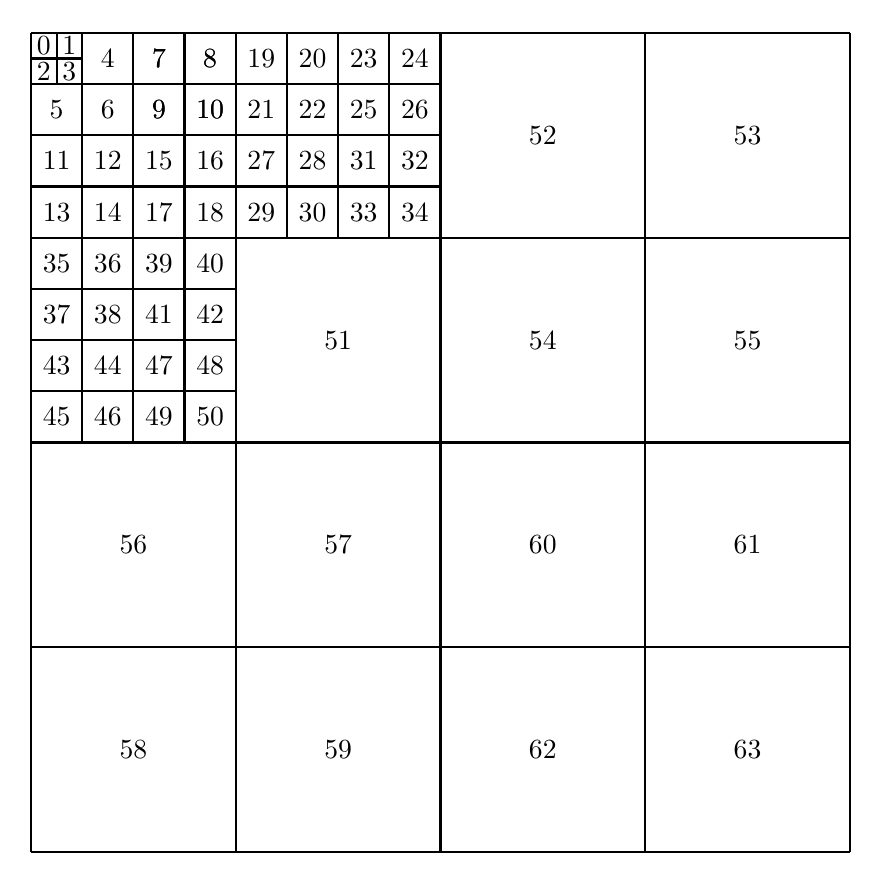
\begin{tikzpicture}[scale=.65]
\draw [draw, step=1cm, thick] (0,8) grid (4,12);
\draw[draw, thick, step=1cm] (0,12) grid (8,16);
\draw[step=4cm, thick, draw](0,0) grid (16,16);
\draw[draw, step=.5,thick](0,15)grid(1,16);

\foreach \x in {0, 1} {
\foreach \y [evaluate=\y as \r using int((\x)+2*(\y))] in {0, 1}{

\node[draw=none]()at(.25+.5*\x,15.75-.5*\y){\r};
	};
	};

\node[draw=none]()at(1.5, 15.5){4};
\node[draw=none]()at(.5,14.5){5};
\node[draw=none]()at(1.5,14.5){6};


\foreach \x in {0, 1} {
\foreach \y [evaluate=\y as \r using int((\x)+2*(\y) + 7)] in {0, 1}{

\node[draw=none]()at(2.5+1*\x,15.5-1*\y){\r};
	};
	};

\foreach \x in {0, 1} {
\foreach \y [evaluate=\y as \r using int((\x)+2*(\y) + 7)] in {0, 1}{

\node[draw=none]()at(2.5+1*\x,15.5-1*\y){\r};
	};
	};

\foreach \x in {0, 1} {
\foreach \y [evaluate=\y as \r using int((\x)+2*(\y) + 11)] in {0, 1}{

\node[draw=none]()at(.5+1*\x,13.5-1*\y){\r};
	};
	};

\foreach \x in {0, 1} {
\foreach \y [evaluate=\y as \r using int((\x)+2*(\y) + 15)] in {0, 1}{

\node[draw=none]()at(2.5+1*\x,13.5-1*\y){\r};
	};
	};



\foreach \j in {0, 1} {
\foreach \k in {0, 1} {
\foreach \x in {0, 1} {
\foreach \y [evaluate=\y as \r using int((\x)+2*(\y) + 4*(\j) + 8*(\k)+ 19)] in {0, 1}{

\node[draw=none]()at(4.5+2*\j+1*\x,15.5-2*\k-1*\y){\r};
	};
	};
    };
    };

\foreach \j in {0, 1} {
\foreach \k in {0, 1} {
\foreach \x in {0, 1} {
\foreach \y [evaluate=\y as \r using int((\x)+2*(\y) + 4*(\j) + 8*(\k)+ 35)] in {0, 1}{

\node[draw=none]()at(.5+2*\j+1*\x,11.5-2*\k-1*\y){\r};
	};
	};
    };
    };

\node[draw=none]()at(6,10){51};

\foreach \x in {0, 1} {
\foreach \y [evaluate=\y as \r using int((\x)+2*(\y) + 60)] in {0, 1}{

\node[draw=none]()at(10+4*\x,6-4*\y){\r};
	};
	};

\foreach \x in {0, 1} {
\foreach \y [evaluate=\y as \r using int((\x)+2*(\y) + 56)] in {0, 1}{

\node[draw=none]()at(2+4*\x,6-4*\y){\r};
	};
	};

\foreach \x in {0, 1} {
\foreach \y [evaluate=\y as \r using int((\x)+2*(\y) + 52)] in {0, 1}{

\node[draw=none]()at(10+4*\x,14-4*\y){\r};
	};
	};

\end{tikzpicture}
\caption{Subband Pattern for WSQ.}
\label{fig:subbands}
\end{figure}
We need to calculate the subband pattern found in Figure \ref{fig:subbands}.
This subband pattern is somewhat arbitrary, but is used because of its empirically good results in compression.
While the pattern may appear complicated at first, we can obtain the
required subband coefficients rather easily.
To start, decompose the image
into 16 subbands, first by using the \li{dwt2} function to split the
image into four subbands, and then applying the function again to each of the
four subbands.
We give a reference implementation of a function that accomplishes just this task, together with its inverse, below:
\begin{lstlisting}
def _decompose16(self, image, wavelet):
    """
    Decompose an array into 16 subbands.

    Parameters
    ----------
    image : numpy array to be decomposed.
    wavelet : string, giving the pywavelets name of the wavelet to use

    Returns
    -------
    subbands : list of 16 numpy arrays giving the subbands
    """
    subbands = []
    LL, HVD = pywt.dwt2(image, wavelet, mode='per')
    dec = pywt.dwt2(LL, wavelet, mode='per')
    subbands.append(dec[0])
    subbands.extend(dec[1])
    for i in xrange(3):
        dec = pywt.dwt2(HVD[i], wavelet, mode='per')
        subbands.append(dec[0])
        subbands.extend(dec[1])
    return subbands
def _recreate16(self, subbands, wavelet):
    """
    Recreate the original from the 16 subbands.

    Parameters
    ----------
    subbands : list of 16 numpy arrays giving the subbands
    wavelet : string, giving the pywavelets name of the wavelet to use

    Returns
    -------
    img : numpy array, inverting the effect of _decompose16
    """
    LL = pywt.idwt2((subbands[0], tuple(subbands[1:4])), wavelet, mode='per')
    details = []
    for i in xrange(1,4):
        details.append(pywt.idwt2((subbands[4*i], tuple(subbands[4*i+1:4*i+4])), wavelet, mode='per'))
    return pywt.idwt2((LL, tuple(details)), wavelet, mode='per')
\end{lstlisting}

Using the function \li{_decompose16} on the fingerprint image,
you should now have a grid of 16 subbands.
Next, split each of the three subbands found in the top left corner of the subband
grid into 16 additional subbands, in the same way as before. You now have a grid
of $13 + 3(16) = 61$ subbands.

Finally, take the very top left subband, and split this into four additional subbands.
You should have 64 subbands. Place them into a list in the order indicated by
the numbers in Figure \ref{fig:subbands}.

\begin{problem}
Implement the subband decomposition as described above by adding a class method \li{_decompose}.
We give an implementation below. Insert comments to demonstrate your understanding of the code.
\begin{lstlisting}
def _decompose(self, img):
    """
    Decompose an image into the WSQ subband pattern.

    Parameters
    ----------
    img : numpy array holding the image to be decomposed

    Returns
    -------
    subbands : list of 64 numpy arrays containing the WSQ subbands in order
    """
    wavelet='coif1'
    subbands = []
    # insert comment
    temp1 = self._decompose16(img, wavelet)

    # insert comment
    temp2 = []
    for i in xrange(3):
        temp2.append(self._decompose16(temp1[i], wavelet))

    # insert comment
    ll, hvd = pywt.dwt2(temp2[0][0], wavelet, mode='per')

    # insert comment
    subbands.append(ll)
    subbands.extend(hvd)
    subbands.extend(temp2[0][1:])
    subbands.extend(temp2[1])
    subbands.extend(temp2[2])
    subbands.extend(temp1[3:])
    return subbands
\end{lstlisting}

Implement the inverse of this decomposition as well, i.e. write code that will take
a list of the 64 subbands and reproduce the original image.
Below we give an implementation.
Again, insert comments.
\begin{lstlisting}
def _recreate(self, subbands):
    """
    Recreate an image from the 64 WSQ subbands.

    Parameters
    ----------
    subbands : list of 64 numpy arrays containing the WSQ subbands in order

    Returns
    -------
    img : numpy array, the recreated image
    """
    wavelet='coif1'
    # insert comment
    ll = pywt.idwt2((subbands[0], tuple(subbands[1:4])), wavelet, mode='per')
    temp1 = []
    temp2 = []
    temp2.append(ll)
    temp2.extend(subbands[4:19])
    # insert comment
    temp1.append(self._recreate16(temp2, wavelet))
    temp1.append(self._recreate16(subbands[19:35], wavelet))
    temp1.append(self._recreate16(subbands[35:51], wavelet))
    temp1.extend(subbands[51:])
    # insert comment
    img = self._recreate16(temp1, wavelet)
    return img
\end{lstlisting}

Implement the next step in the \li{compress} method by calculating the wavelet subbands using \li{_decompose}.
\end{problem}

\subsection*{WSQ: Quantization}
Quantization is the process of mapping each wavelet coefficient to an
integer value, and is the main source of compression in the algorithm.
By mapping
the wavelet coefficients to a relatively small set of integer values, we reduce
the complexity of the data, which will allow us to efficiently encode the information
in a bit string. Further, a large portion of the wavelet coefficients will be mapped to 0
and discarded completely.
The fact that fingerprint images tend to be very nearly sparse in the wavelet domain
means that we don't lose too much information from quantization.
We must take care, however, to perform this quantization in a
manner that achieves good compression without discarding so much information that we
are unable to reconstruct the image accurately.

Given a wavelet coefficient $a$ in subband $k$, the corresponding quantized
coefficient $p$ is given by
\[
p =
\begin{cases}
   \left\lfloor\frac{a-Z_k/2}{Q_k}\right\rfloor + 1, & a> Z_k/2 \\
   0,       & -Z_k/2 \leq a \leq Z_k/2\\
   \left\lceil\frac{a + Z_k/2}{Q_k}\right\rceil - 1, & a < -Z_k/2
  \end{cases}
\]
The values $Z_k$ and $Q_k$ are dependent on the subband, and determine how much
compression is achieved.
If $Q_k=0$, we simply map the coefficient to 0.

Selecting appropriate values for these parameters is a tricky problem in itself, and relies on heuristics
based on the statistical properties of the wavelet coefficients.
Therefore, we provide you with a method to come up with these values.
The method accepts the list of subbands as well as the parameters \li{r} and \li{gamma}
that were passed to the \li{compress} method, and returns arrays $Q$ and $Z$,
which give $Q_k$ and $Z_k$ for subbands $k=0,\ldots,63$.
\begin{lstlisting}
def _getBins(self, subbands, r, gamma):
    """Calculate quantization bin widths for each subband."""
    subband_vars = np.zeros(64)
    fracs = np.zeros(64)
    for i in xrange(len(subbands)): # compute subband variances
        X,Y = subbands[i].shape
        fracs[i]=(X*Y)/(np.float(finger.shape[0]*finger.shape[1]))
        x = np.floor(X/8.)
        y = np.floor(9*Y/32.)
        Xp = np.floor(3*X/4.)
        Yp = np.floor(7*Y/16.)
        mu = subbands[i].mean()
        sigsq = (Xp*Yp-1.)**(-1)*((subbands[i][x:x+Xp, y:y+Yp]-mu)**2).sum()
        subband_vars[i] = sigsq

    A = np.ones(64)
    A[52], A[56] = [1.32]*2
    A[53], A[58], A[55], A[59] = [1.08]*4
    A[54], A[57] = [1.42]*2

    Qprime = np.zeros(64)
    mask = subband_vars >= 1.01
    Qprime[mask] = 10./(A[mask]*np.log(subband_vars[mask]))
    Qprime[:4] = 1
    Qprime[60:] = 0

    K = []
    for i in xrange(60):
        if subband_vars[i] >= 1.01:
            K.append(i)

    while True:
        S = fracs[K].sum()
        P = ((np.sqrt(subband_vars[K])/Qprime[K])**fracs[K]).prod()
        q = (gamma**(-1))*(2**(r/S-1))*(P**(-1./S))
        E = []
        for i in K:
            if Qprime[i]/q >= 2*gamma*np.sqrt(subband_vars[i]):
                E.append(i)
        if len(E) > 0:
            for i in E:
                K.remove(i)
            continue
        break

    Q = np.zeros(64) # final bin widths
    for i in K:
        Q[i] = Qprime[i]/q
    Z = 1.2*Q

    return Q, Z
\end{lstlisting}

Quantization is not a perfectly invertible process. Once we have quantized
the wavelet coefficients, some information is permanently lost. However, we can
roughly reconstruct the wavelet coefficients $\hat{a}_k$ in subband $k$ from the quantized coefficients
$p$ using the following formula.
This process is called \emph{dequantization}.
\[
\hat{a}_k =
\begin{cases}
(p-C)Q_k + Z_k/2, & p> 0\\
0, & p = 0\\
(p + C)Q_k - Z_k/2, & p < 0
\end{cases}
\]
For our purposes, take $C = 0.44$. Again, if $Q_k = 0$, just return $\hat{a}_k = 0$.
\begin{problem}
Implement the quantization step by adding the following method to your class:
\begin{lstlisting}
def _quantize(self, coeffs, Q, Z):
    """
    Implement a uniform quantizer.

    Parameters
    ----------
    coeffs : numpy array containing the floating-point values to be quantized.
    Q : the step size of the quantization, a nonnegative float
    Z : the null-zone width (of the center/0 quantization bin) nonnegative float

    Returns
    -------
    out : numpy array of same shape as coeffs holding the quantized values
    """
    pass
\end{lstlisting}
Wherever possible, operate on the vectors as a whole rather than writing for-loops.
You may wish to make use of the array slicing techniques demonstrated below:
\begin{lstlisting}
>>> # assume X, Y are numpy arrays of same shape
>>> m = X < -2 # create mask for entries less than -2
>>> Y[m] = np.ceil(X[m]) + 2 # set corresponding entries of Y
\end{lstlisting}

Implement the dequantization step as well.
\begin{lstlisting}
def _dequantize(self, coeffs, Q, Z, C=0.44):
    """
    Reverse the quantization effect (approximately).

    Parameters
    ----------
    coeffs : numpy array of quantized coefficients
    Q : see doc for quantize
    Z : see doc for quantize
    C : centering parameter

    Returns
    -------
    out : array of dequantized coefficients, same shape as coeffs
    """
    pass
\end{lstlisting}
Remember to consider the case where $Q=0$!

Observe that both quantization and dequantization require $Q_k$ and $Z_k$ for each subband $k$.
Thus, once you obtain these values in the \li{compress} method using \li{_getBins}, store them in the class attributes
\li{_Q} and \li{_Z}.
Then, calculate the 64 compressed subbands.
For example, if \li{subbands} is a list containing the 64 wavelet subbands, the following
code will produce a list of the quantized subbands:
\begin{lstlisting}
>>> # get the quantization parameters, store
>>> self._Q, self._Z = self._getBins(subbands, r, gamma)
>>> # now create a list of all quantized subbands
>>> q_subbands = [self._quantize(subbands[i],self._Q[i],self._Z[i]) for i in xrange(64)]
\end{lstlisting}
\end{problem}
\subsection*{WSQ: Grouping}
At this point in the algorithm, we have a list of 64 arrays, where the $k$-th
entry is a matrix containing the quantized wavelet coefficients for the $k$-th subband.
The remaining steps in the algorithm focus on entropy coding these quantized
coefficients to further increase compression.
As such, we have finished with the wavelet analysis portion.

We will segment the list of quantized subbands into three groups.
This gives three lists of quantized coefficients, each having a high degree of homogeneity.
This is important for the entropy coding, since we can achieve better compression by separately encoding groups of similar coefficients.

Group quantized subbands $0$ through $18$ together, $19$ through $51$ together, and finally $52$ through $63$ together.
You may understand the logic of these groupings when glancing back at Figure \ref{fig:subbands}.
When grouping subbands together, flatten each subband and concatenate their entries together, so that you obtain a simple list of integer values.
Since we are flattening and then concatenating the subbands, we need to save the shape of the original subbands, so that we can later
reconstruct the subbands from the groups of coefficients.
Finally, we will not include subbands that consist entirely of zeros, as these contain no information and thus don't need to be stored.
Therefore, while looping through the subbands and creating the lists of coefficients, include a check for nonzero entries in the subband,
and also create a list of boolean values for each group whose $i$-th entry indicates whether the $i$-th subband in the group was included.

Below is sample code for producing the first group.
Use a similar approach for the other two groups.
\begin{lstlisting}
>>> # assume subbands is my list of the 64 quantized subbands
>>> g1 = []     # this will hold the group 1 coefficients
>>> s1 = []     # keep track of the subband dimensions in group 1
>>> t1 = []     # keep track of which subbands were included
>>> for i in xrange(19):
>>>     s1.append(subbands[i].shape)
>>>     if subbands[i].any(): # True if any nonzero entry
>>>         g1.extend(subbands[i].ravel())
>>>         t1.append(True)
>>>     else: # the subband was not transmitted
>>>         t1.append(False)
\end{lstlisting}

To reconstruct the subbands from \li{g1}, \li{s1}, and \li{t1}, we have the following code:
\begin{lstlisting}
>>> # reconstruct the subbands in group 1
>>> subbands1 = []     # the reconstructed subbands in group 1
>>> i = 0
>>> for j, shape in enumerate(s1):
>>>     if t1[j]: # if the j-th subband was included
>>>         l = shape[0]*shape[1] # number of entries in the subband
>>>         subbands1.append(np.array(g1[i:i+l]).reshape(shape))
>>>         i += l
>>>     else: # the j-th subband wasn't included, so all zeros
>>>         subbands1.append(np.zeros(shape))
\end{lstlisting}
\begin{problem}
Carry out the grouping procedure and its inverse as described above by implementing
the following class methods:
\begin{lstlisting}
def _group(self, subbands):
    """
    Split the quantized subbands into 3 groups.

    Parameters
    ----------
    subbands : list of 64 numpy arrays containing quantized coefficients

    Returns
    -------
    gs : tuple (g1,g2,g3)
         each gi a list of quantized coeffs for groups i
    ss : tuple (s1,s2,s3)
         each si a list of tuples, the shapes of the subbands in group i
    ts : tuple (t1,t2,t3)
         each ti a list of bools indicating which subbands included
    """
    pass

def _ungroup(self, gs, ss, ts):
    """
    Re-create the subband list structure from the three groups.

    Parameters
    ----------
    gs : tuple of form (g1, g2, g3)
    ss : tuple of form (s1, s2, s3)
    ts : tuple of form (t1, t2, t3)
    See the docstring for _group.

    Returns
    -------
    subbands : list of 64 numpy arrays
    """
    pass
\end{lstlisting}

Note that we need the shapes and the boolean lists indicating which subbands were included
for the un-grouping step.
Thus, in the \li{compress} method, once we computed these tuples of lists, we store them in the class attributes \li{_shapes}
and \li{_tvals}, respectively.
\begin{lstlisting}
>>> groups, self._shapes, self._tvals = self._group(q_subbands)
\end{lstlisting}
\end{problem}

\subsection*{WSQ: From Quantized Coefficients to Huffman Indices}
We now have three groups of integer-valued quantized coefficients.
It remains to encode each of these three groups using Huffman coding.

Note that each group is likely to contain many consecutive zeros, since we have rounded all of the smallest
wavelet coefficients to zero.
There will also be a few quantized coefficients of high magnitude.
The remaining nonzero coefficients will have values between $-73$ and $74$.
With this in mind, we can represent these groups of coefficients even more tersely by
mapping them to a set of discrete values (integers from $0$ to $253$), which we call \emph{Huffman Indices}.
The mapping between Huffman indices and quantized coefficients is given in Table \ref{table:huffIndex}.
\begin{table}
\begin{tabular}{|c|c|}
\hline
\textbf{Huffman Index} & \textbf{Quantized Coefficient}\\\hline
0 & zero run length 1\\\hline
1 & zero run length 2\\\hline
\vdots & \vdots\\\hline
99 & zero run length 100\\\hline
100 & $75\leq q \leq 255$\\\hline
101 & $-255 \leq q \leq -74$\\\hline
102 & $256 \leq q \leq 65535$\\\hline
103 & $-65535 \leq q \leq -256$\\\hline
104 & zero run of length $101\leq n \leq 255$\\\hline
105 & zero run of length $255\leq n \leq 65535$\\\hline
106 & -73\\\hline
107 & -72\\\hline
108 & -71\\\hline
\vdots & \vdots\\\hline
179 & 0 \emph{(use index 0)}\\\hline
\vdots & \vdots \\\hline
252 & 73\\\hline
253 & 74\\\hline
\end{tabular}
\caption{The mapping between Huffman indices and quantized coefficients.}
\label{table:huffIndex}
\end{table}

To see how this mapping works, suppose that we have the following list of quantized coefficients:
\[
[0, 0, 0, 0, -45, 13, 103, -269, 0]
\]
The list starts off with a zero run of length $4$, so the first Huffman index is $3$
(each zero run of length $n$ where $n\leq 100$ get a Huffman index of $n-1$).
The next coefficient is $-45$, so we infer from the Table that its Huffman index
is $-45 + (106+73) = 134$.
The next coefficient is $13$, so as before, its Huffman index is $13 + 179 = 192$.
The final three indices are $100$, $103$, and $0$.

Note that this mapping is not one-to-one when dealing with zero runs of lengths greater than $100$,
or with coefficients of sufficiently large magnitudes (the Huffman indices for these cases
are 100 through 105).
We refer to these cases as \emph{exceptional cases}.
When we encounter exceptional cases, we need to
store the length of the zero run or the magnitude of the coefficient, so that we can perfectly
reconstruct the quantized coefficients at the decompression stage.
Hence, while generating a list of the Huffman indices for each group, we also generate a list
of extra values for the exceptional cases.

Finally, as we generate the list of Huffman indices from the quantized coefficients, we also tabulate
the frequency of each index, as this is necessary when building a Huffman Encoder.

Below we give code to calculate the Huffman indices, frequencies, and extra values given a list of
quantized coefficients.
\begin{lstlisting}
def _huffmanIndices(self, coeffs):
    """
    Calculate the Huffman indices from the quantized coefficients.

    Parameters
    ----------
    coeffs : list of integer values

    Returns
    -------
    inds : list of Huffman indices
    freqs : numpy array whose i-th entry gives frequency of index i
    extra : list of zero run lengths or coefficient magnitudes for exceptional cases
    """
    N = len(coeffs)
    i = 0
    inds = []
    extra = []
    freqs = np.zeros(254)

    # sweep through the quantized coefficients
    while i < N:
        # first handle zero runs
        zero_count = 0
        while coeffs[i] == 0:
            zero_count += 1
            i += 1
            if i >= N:
                break
        if zero_count > 0 and zero_count < 101:
            inds.append(zero_count - 1)
            freqs[zero_count - 1] += 1
        elif zero_count >= 101 and zero_count < 256: # 8 bit zero run
            inds.append(104)
            freqs[104] += 1
            extra.append(zero_count)
        elif zero_count >= 256: # 16 bit zero run
            inds.append(105)
            freqs[105] += 1
            extra.append(zero_count)
        if i >= N:
            break
        # now handle nonzero coefficients
        if coeffs[i] > 74 and coeffs[i] < 256: # 8 bit pos coeff
            inds.append(100)
            freqs[100] += 1
            extra.append(coeffs[i])
        elif coeffs[i] >= 256: # 16 bit pos coeff
            inds.append(102)
            freqs[102] += 1
            extra.append(coeffs[i])
        elif coeffs[i] < -73 and coeffs[i] > -256: # 8 bit neg coeff
            inds.append(101)
            freqs[101] += 1
            extra.append(abs(coeffs[i]))
        elif coeffs[i] <= -256: # 16 bit neg coeff
            inds.append(103)
            freqs[103] += 1
            extra.append(abs(coeffs[i]))
        else: # current value is a nonzero coefficient in the range [-73, 74]
            inds.append(179 + coeffs[i])
            freqs[179 + coeffs[i]] += 1
        i += 1
    return inds, freqs, extra
\end{lstlisting}
\begin{problem}
Examine the code for \li{_huffmanIndices} to make sure you understand it, and add it to your class.
\end{problem}

In the decompression stage, we need to recover the quantized coefficients from the Huffman Indices.
As noted before, the mapping is not one-to-one for the exceptional cases, so we need both the list
of indices and the extra values.
Given these two lists, it is not difficult to recover the coefficients.
\begin{lstlisting}
def _indicesToCoeffs(self, indices, extra):
    """
    Calculate the coefficients from the Huffman indices plus extra values.

    Parameters
    ----------
    indices : list of integer values (Huffman indices)
    extra : list of indices corresponding to values with exceptional indices

    Returns
    -------
    coeffs : list of quantized coefficients recovered from the indices.
    """
    coeffs = []
    j = 0 # index for extra array
    for s in indices:
        if s < 100: # zero count of 100 or less
            coeffs.extend(np.zeros(s+1))
        elif s == 104 or s == 105: # zero count of 8 or 16 bits
            coeffs.extend(np.zeros(extra[j]))
            j += 1
        elif s in [100, 102]: # 8 or 16 bit pos coefficient
            coeffs.append(extra[j]) # get the coefficient from the extra list
            j += 1
        elif s in [101, 103]: # 8 or 16 bit neg coefficient
            coeffs.append(-extra[j]) # get the coefficient from the extra list
            j += 1
        else: # coefficient from -73 to +74
            coeffs.append(s-179)
    return coeffs
\end{lstlisting}
\begin{problem}
Examine the code for \li{_indicesToCoeffs} for understanding, and then add the method to your class.
\end{problem}
\subsection*{Reading and Writing Bits with bitstring}
In the final stage of the algorithm, we take our lists of Huffman indices and map them to bit patterns.
Pure Python is not equipped to manipulate data
at the bit level, so we will use the Python package \li{bitstring} to facilitate the process.
In this section we present the functions required for the WSQ algorithm.

Once you have installed the package, type the import command:
\begin{lstlisting}
>>> import bitstring as bs
\end{lstlisting}
In order to build a string of bits, we initialize a \li{BitArray} object, and then add the
desired bit patterns.
\begin{lstlisting}
>>> bits = bs.BitArray()
>>> # add bit patters 1101 and 01
>>> bits.append('0b1101')
>>> bits.append('0b01')
\end{lstlisting}
Note that the string containing the bit pattern must begin with \li{'0b'}.

We can add an 8- or 16-bit representations of an integer as follows:
\begin{lstlisting}
>>> # add the 8-bit integer 212, and then the 16-bit integer 1047
>>> bits.append('uint:8=212')
>>> bits.append('uint:16=1047')
\end{lstlisting}
To view the bits contained in the \li{BitArray}, we can print the \li{bin} attribute.
\begin{lstlisting}
>>> # view the entire bit string
>>> print bits.bin
110101110101000000010000010111
\end{lstlisting}

When reading the data from a bit stream, we use a \li{bs.ConstBitStream} object, and call its \li{read} method, giving it an input string
that specifies the way to interpret the bits, and the number of bits to read.
To read the next 3 bits as binary, the input string would be \li{'bin:3'}, whereas to read the next 16 bits as an unsigned integer
you would provide the input string \li{'uint:16'}.
Let's read the first 6 bits of \li{bits}, one at a time:
\begin{lstlisting}
>>> bitreader = bs.ConstBitStream(bits)
>>> for i in xrange(6):
>>>     print bitreader.read('bin:1')
1
1
0
1
0
1
\end{lstlisting}
We know that the next 8 bits should be interpreted as an unsigned integer, and likewise for the
following 16 bits. Thus, we read these bits as follows:
\begin{lstlisting}
>>> print bitreader.read('uint:8')
212
>>> print bitreader.read('uint:16')
1047
\end{lstlisting}

You now have all the tools necessary to read and write the compressed image bit stream.

\subsection*{WSQ: Huffman Coding}
Huffman coding is a technique for assigning binary codes to a collection of symbols in such a way
that minimizes the total number of bits needed to encode the symbols.
More frequent symbols will be assigned shorter binary codes, while rare symbols will have
longer codes.
One simple way to implement Huffman Coding is to build a binary tree, whose leaves correspond
to the different symbols to be encoded.
We then traverse the tree from the root down to each leaf node to generate the binary codes
(left corresponds to 0, right corresponds to 1).
Below we give a reference implementation.
\begin{lstlisting}
import Queue
class huffmanLeaf():
    """Leaf node for Huffman tree."""
    def __init__(self, symbol):
        self.symbol = symbol
    def makeMap(self, huff_map, path):
        huff_map[self.symbol] = path

class huffmanNode():
    """Internal node for Huffman tree."""
    def __init__(self, left, right):
        self.left = left
        self.right = right
    def makeMap(self, huff_map, path):
        """
        Traverse the huffman tree to build the encoding map.
        """
        self.left.makeMap(huff_map, path + '0')
        self.right.makeMap(huff_map, path + '1')

def huffman(freqs):
    """
    Generate the huffman tree for the given symbol frequencies.
    Return the map from symbol to bit pattern.
    """
    q = Queue.PriorityQueue()
    for i in xrange(len(freqs)):
        leaf = huffmanLeaf(i)
        q.put((freqs[i], leaf))
    while q.qsize() > 1:
        l1 = q.get()
        l2 = q.get()
        weight = l1[0] + l2[0]
        node = huffmanNode(l1[1], l2[1])
        q.put((weight,node))
    root = q.get()[1]
    huff_map = dict()
    root.makeMap(huff_map, '')
    return huff_map
\end{lstlisting}
When we pass a list of Huffman indices to the function \li{huffman}, we obtain
obtain a dictionary (called the Huffman map) whose keys are the integers 0 through 253 (the Huffman indices)
and whose values are the bit pattern assigned to each Huffman index.
This Huffman map, together with the list of Huffman indices and extra values,
allows us to encode the quantized coefficients as a bit string.
Make sure you understand the implementation of the encoding process given below:
\begin{lstlisting}
def _encode(self, indices, extra, huff_map):
    """
    Encode the indices using the Huffman map, return the resulting bitstring.

    Parameters
    ----------
    indices : list of integer values, the Huffman Indices
    extra : list of integer coefficients corresponding to exceptional indices
    huff_map : dict that maps Huffman index to bit pattern

    Returns
    -------
    bits : BitArray object containing bit representation of the Huffman indices
    """
    bits = bs.BitArray()
    j = 0 # index for extra array
    for s in indices: # encode each huffman index
        bits.append('0b' + huff_map[s])

        # encode extra values for exceptional cases
        if s in [104, 100, 101]: # encode as 8-bit ints
            bits.append('uint:8={}'.format(int(extra[j])))
            j += 1
        elif s in [102, 103, 105]: # encode as 16-bit ints
            bits.append('uint:16={}'.format(int(extra[j])))
            j += 1
    return bits
\end{lstlisting}

\begin{problem}
Add the \li{_encode} method to your class.
Implement the Huffman coding step in the \li{compress} method by calculating
the Huffman indices, Huffman map, and bit string for each group of quantized coefficients separately.
Store the resulting three bit strings and Huffman maps in the class attributes \li{_bitstrings}
and \li{_huff_maps}.
Use the following code block as a guide.
\begin{lstlisting}
>>> # assume groups is a list of the three groups of coefficients
>>> # for each group, get huffman indices, create huffman tree, and encode
>>> huff_maps = []
>>> bitstrings = []
>>> for i in xrange(3):
>>>     inds, freqs, extra = self._huffmanIndices(groups[i])
>>>     huff_map = huffman(freqs)
>>>     huff_maps.append(huff_map)
>>>     bitstrings.append(self._encode(inds, extra, huff_map))
>>>
>>> # store the bitstrings and the huffman maps
>>> self._bitstrings = bitstrings
>>> self._huff_maps = huff_maps
\end{lstlisting}
You have now fully implemented the compression algorithm!
\end{problem}

For decompression, we need to decode the bit strings back to Huffman indices.
This is straight-forward enough using the Huffman maps.
Essentially, we read the bit string one bit at a time, check to see if we have a bit pattern
found in the Huffman map, and if so, store the corresponding Huffman index in the list of Huffman indices.
If the Huffman index is an exceptional case, we read the next 8 or 16 bits from
the bit string (depending on the exact value of the index), and store the resulting
value in the list of extra values.
Examine the implementation below for understanding:
\begin{lstlisting}
def _decode(self, bits, huff_map):
    """
    Decode the bits using the given huffman map, return the resulting indices.

    Parameters
    ----------
    bits : BitArray object containing the bit-encoded indices
    huff_map : dict that maps huffman index to bit pattern

    Returns
    -------
    indices : list of decoded huffman indices
    extra : list of decoded values corresponding to exceptional indices
    """
    indices = []
    extra = []

    # reverse the huffman map to get the decoding map
    dec_map = {v:k for k, v in huff_map.items()}

    # wrap the bits in an object better suited to reading
    bits = bs.ConstBitStream(bits)

    # read each bit at a time, decoding as we go
    i = 0 # the index of current bit
    pattern = '' # the current bit pattern
    while i < bits.length:
        pattern += bits.read('bin:1') # read in another bit
        i += 1

        # check if current pattern is in the decoding map
        if dec_map.has_key(pattern):
            indices.append(dec_map[pattern]) # insert huffman index

            # if an exceptional index, read next bits for extra value
            if dec_map[pattern] in (100, 101, 104): # 8-bit int or 8-bit zero run length
                extra.append(bits.read('uint:8'))
                i += 8
            elif dec_map[pattern] in (102, 103, 105): # 16-bit int or 16-bit zero run length
                extra.append(bits.read('uint:16'))
                i += 16
            pattern = '' # reset the bit pattern
    return indices, extra
\end{lstlisting}

\begin{problem}
Add the \li{_decode} method to your class.
\end{problem}

\subsection*{WSQ: Decompression}
Decompression refers to recovering the original image from the bit encodings of the quantized wavelet coefficients.
You already have all of the methods required for decompression; what remains is to put them together.
Make sure you understand what's going on in the following implementation.
\begin{lstlisting}
def decompress(self):
    """
    Return the uncompressed image recovered from the compressed bistring representation.

    Returns
    -------
    img : numpy array giving the recovered uncompressed image.
    """
    # for each group, decode the bits, map from indices to coefficients
    groups = []
    for i in xrange(3):
        indices, extras = self._decode(self._bitstrings[i], self._huff_maps[i])
        groups.append(self._indicesToCoeffs(indices, extras))

    # recover the subbands from the groups of coefficients
    q_subbands = self._ungroup(groups, self._shapes, self._tvals)

    # dequantize the subbands
    subbands = [self._dequantize(q_subbands[i], self._Q[i], self._Z[i]) for i in xrange(64)]

    # recreate the image
    img = self._recreate(subbands)

    # post-process, return the image
    return self._postProcess(img)
\end{lstlisting}
\begin{problem}
Add the \li{decompress} method to your class.
\end{problem}

\subsection*{WSQ: Calculating the Compression Ratio}
The compression ratio is the ratio of the number of bits in the original image to the number of bits in the encoding.
Assuming that each pixel of the input image is an 8-bit integer, the number of bits in the image is just 8 times the number of pixels
(recall that the number of pixels in the original source image is stored in the class attribute \li{_pixels}).
We can calculate the number of bits in the encoding by adding up the lengths of each of the three bit strings stored
in the class attribute \li{_bitstrings}.
\begin{problem}
Add the method \li{getRatio} to your class by implementing the following:
\begin{lstlisting}
def getRatio(self):
    """
    Calculate the compression ratio achieved.

    Returns
    -------
    ratio : float, the ratio of number of bytes in original image to number of bytes contained
            in the three bitstrings combined.
    """
    pass
\end{lstlisting}
Watch out for integer division!
\end{problem}

We now have a fully functional implementation of the Wavelet Scalar Quantization algorithm for image compression.
Test out your code by compressing the fingerprint image finger.pgm for different values of $r$ (say in the range
0.1 to 0.9).
Calculate the compression ratio, and plot the original image and compressed image together, as follows:
\begin{lstlisting}
>>> # instantiate a value for r
>>> finger = imread('finger.pgm')
>>> wsq = WSQ()
>>> wsq.compress(finger, r)
>>> print wsq.getRatio()
>>> new_finger = wsq.decompress()
>>> plt.subplot(211)
>>> plt.imshow(finger, cmap=plt.cm.Greys_r)
>>> plt.subplot(212)
>>> plt.imshow(new_finger.clip(finger.min(), finger.max()), cmap=plt.cm.Greys_r)
>>> plt.show()
\end{lstlisting}
\end{comment}


\begin{comment}
We don't need a lot of this expository content in the lab.
\subsection*{The Haar Wavelet}

As noted earlier, the Fourier transform is based on the complex exponential
function. Let us alter the situation and consider instead the following
function, known as the \emph{Haar wavelet}:
\begin{equation*}
\psi(x) =
 \begin{cases}
  1 & \text{if } 0 \leq x < \frac{1}{2} \\
  -1 & \text{if } \frac{1}{2} \leq x < 1 \\
  0 & \text{otherwise.}
 \end{cases}
\end{equation*}

% It might be nice to plot this function and include the image in the lab.

Along with this wavelet, we introduce the associated \emph{scaling function}:
\begin{equation*}
\phi(x) =
 \begin{cases}
 1 & \text{if } 0 \leq x < 1 \\
 0 & \text{otherwise.}
 \end{cases}
\end{equation*}

From the wavelet and scaling function, we can generate two countable families
of dyadic dilates and translates given by
\begin{equation*}
\psi_{m,k}(x) = \psi(2^mx - k)
\end{equation*}
\begin{equation*}
\phi_{m,k}(x) = \phi(2^mx - k),
\end{equation*}
where $m,k \in \mathbb{Z}$.

Let us focus for the moment on that second family of functions, $\{\phi_{m,k}\}$.
If we fix $m$ and let $k$ vary over the integers, we have a countable collection of
simple functions. The support of a typical function $\phi_{m,k}$ is the interval
$[k2^{-m}, (k+1)2^{-m}]$, and for any $m \in \mathbb{Z}$ we have
\begin{equation*}
\mathbb{R} = \displaystyle\biguplus_k\,[k2^{-m}, (k+1)2^{-m}],
\end{equation*}
where $\uplus$ denotes a union over disjoint sets. Thus, the supports can be viewed as
a discretization of the real line, and we can use this collection of simple functions
to approximate any $f \in L^2(\mathbb{R})$ in the following sense:
\begin{equation*}
f(x) \approx f_m(x) := \displaystyle\sum_{k \in \mathbb{Z}}\alpha_{m,k}\phi_{m,k}(x),
\end{equation*}
where
\begin{equation*}
\alpha_{m,k} := 2^m \displaystyle \int_{k2^{-m}}^{(k+1)2^{-m}}f(x) dx
\end{equation*}
($\alpha_{m,k}$ is simply the average value of $f$ on $[k2^{-m},(k+1)2^{-m}]$). As you
would probably expect, the point-wise error between $f$ and its approximation $f_m$
(called a \emph{frame}) goes to zero as $m \to \infty$.

These frames are not quite good enough, however. Each coefficient $\alpha_{m,k}$
certainly captures local information about $f$ -- namely its average value on
a certain interval -- but it fails to tell us anything about how $f$ changes
on that interval. We need more information than is provided by $f_m$ in order
to know about discontinuities or high-frequency oscillations of $f$. To this end,
we now consider the wavelet function $\psi$.
Notice that the Haar wavelet is oscillatory in nature, and is thus better suited
to capture local information on how a function changes at a given point. For
any given $m$, we define a function $d_m$, called a \emph{detail}, as follows:
\begin{equation*}
d_m(x) := \displaystyle\sum_{k \in \mathbb{Z}}\beta_{m,k}\psi_{m,k}(x),
\end{equation*}
where
\begin{equation*}
\beta_{m,k} := 2^m \displaystyle \int_{-\infty}^{\infty}f(x) \psi_{m,k}(x) dx.
\end{equation*}
Each coefficient $\beta_{m,k}$ gives information about how $f$ changes on the
the interval $[k2^{-m}, (k+1)2^{-m}]$, and larger coefficients correspond
to larger spikes of width $2^{-m}$. Thus, as $m$ increases, the
detail function $d_m$ gives information about the higher-frequency oscillations
of the function. The details and approximation frames interact in the following way:
\begin{equation*}
f_{m+1} = f_m + d_m.
\end{equation*}
As a result of this fortuitous relationship, one can prove the decomposition
\begin{equation*}
L^2(R) = V_0 \oplus W_0 \oplus W_1 \oplus \cdots,
\end{equation*}
where $V_j := \text{span}\{\phi_{j,k}\}_{k \in \mathbb{Z}}$ and
$W_j := \text{span}\{\psi_{j,k}\}_{k \in \mathbb{Z}}$. This fact justifies
our hope to approximate and analyze functions using wavelets.
\begin{figure}[t]
\minipage{0.32\textwidth}
    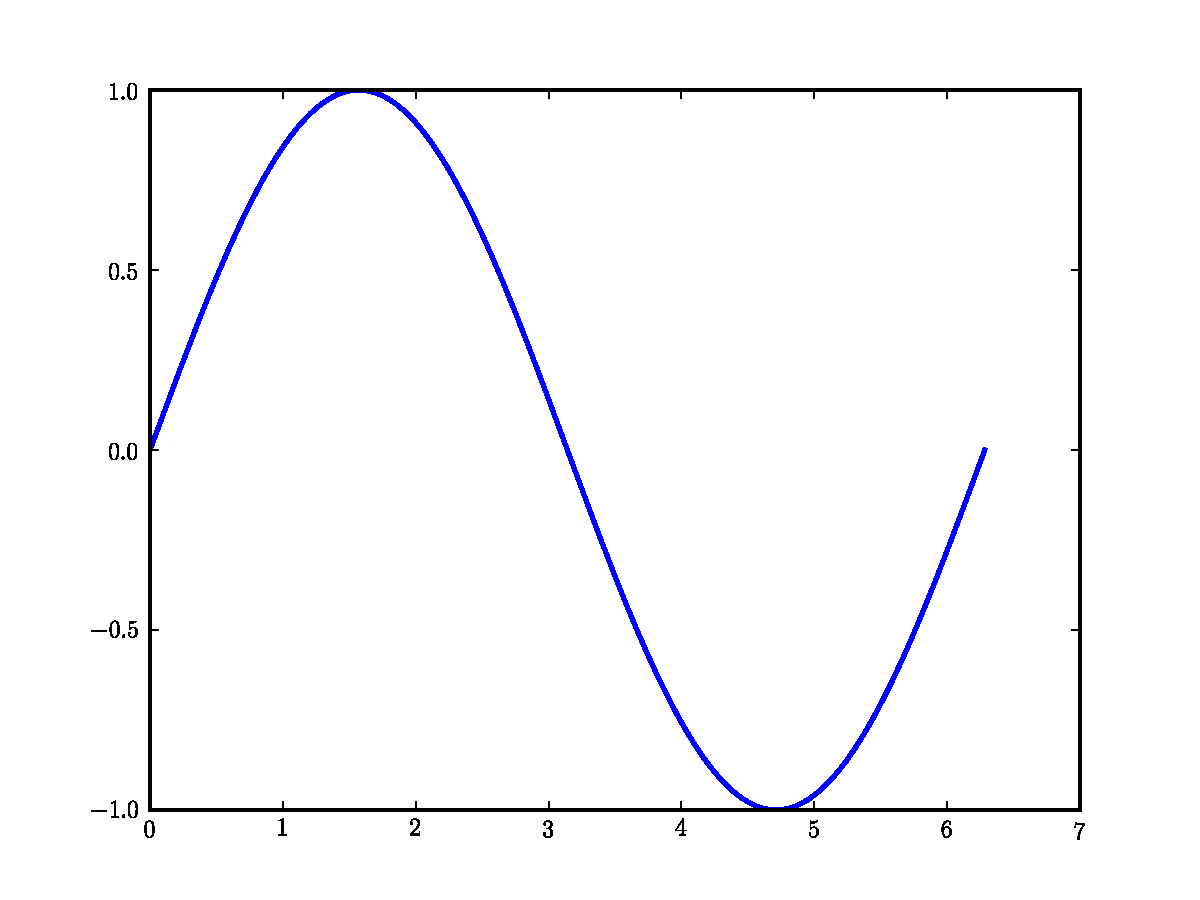
\includegraphics[width=\linewidth]{sinecurve}
    \caption{$f(x) = \sin (x)$}
\endminipage\hfill
\minipage{0.32\textwidth}
    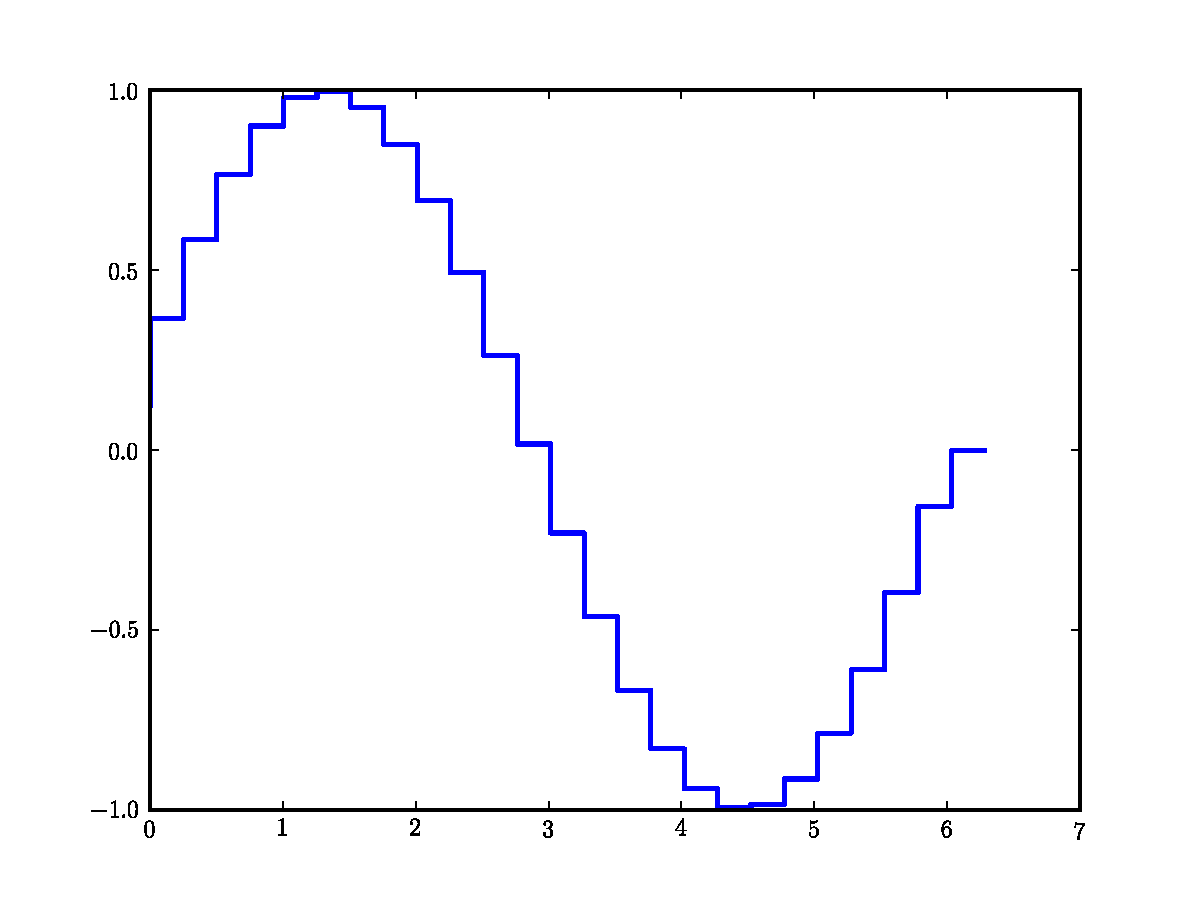
\includegraphics[width=\linewidth]{discreteSineCurve.pdf}
    \caption{$f_4$}
\endminipage\hfill
\minipage{0.32\textwidth}
    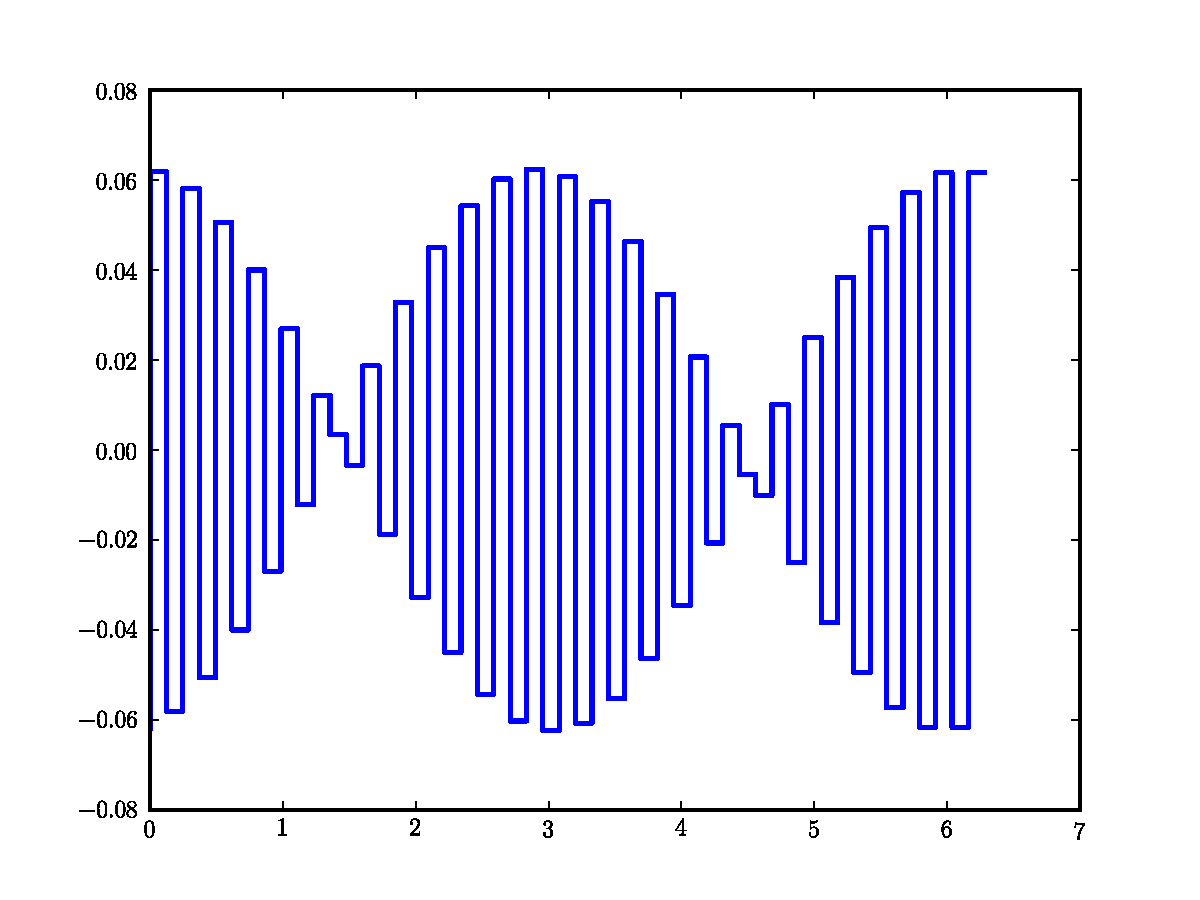
\includegraphics[width=\linewidth]{sineCurveDetail}
    \caption{$d_4$}
\endminipage
\end{figure}
\begin{problem}
Calculate and plot the approximation frames for $f(x) = \sin(x)$ on the interval $[0,2\pi]$
for $m = 4, 6, 8$. Note that because we are working on a finite interval,
we only need to calculate certain coefficients $\alpha_{m,k}$. In
particular, we only need the coefficients for $k = 0$ up to the first integer
$n$ such that $(n+1)2^{-m} > 2 \pi$ (why?). Furthermore, to plot the frame,
all we need is an array containing the relevant coefficients. Then simply plot
the coefficients against \li{linspace} with appropriate arguments
and set \li{drawstyle='steps'} in the \li{plt.plot} function.
\end{problem}

\begin{problem}
Now calculate the details for $f(x) = \sin(x)$ on the same interval and for the
same $m$ values given above. Use previous results to compute the coefficients
for $f_5$, $f_7$, and $f_9$ and plot them.
\end{problem}

What purpose do these details and approximation frames serve? According to the
properties discussed above, we can approximate $L^2$ functions as follows:
\begin{align*}
f \approx f_{J+1} &= f_J + d_J \\
&= f_{J-1} + d_{J-1} + d_J \\
& \ldots\\
&= f_{I} + d_{I} + d_{I+1} + \cdots + d_J,
\end{align*}
where $1 \leq I \leq J$. If $f$ has compact support (as in the case of a finite-time signal,
for example), only finitely many of the coefficients in the frame and the details are
nonzero, thus enabling us to represent $f$ to a reasonable degree of accuracy in a very
efficient manner. The calculation of these detail coefficients is called the \emph{discrete
wavelet transform}. In the context of signals processing, one can imagine calculating these
coefficients, transmitting them, and then reproducing the approximated signal on the
receiving end. Furthermore, the coefficients of the details reflect the local properties
of the original function $f$ at the particular level of detail and resolution! This means
that we can discard many of the coefficients if we are only interested in reproducing a certain
part of the signal, or in recovering the entire signal to only a limited resolution. We can
also study just those frequencies of the signal that fall within a certain range (called a
sub-band) by examining the detail coefficients at a particular level. These
properties make the discrete wavelet transform an attractive alternative to the Fourier
transform in many applications. See Figure \ref{fig:dwt1D} for an example of the discrete Wavelet transform.

\begin{figure}[H]
\centering
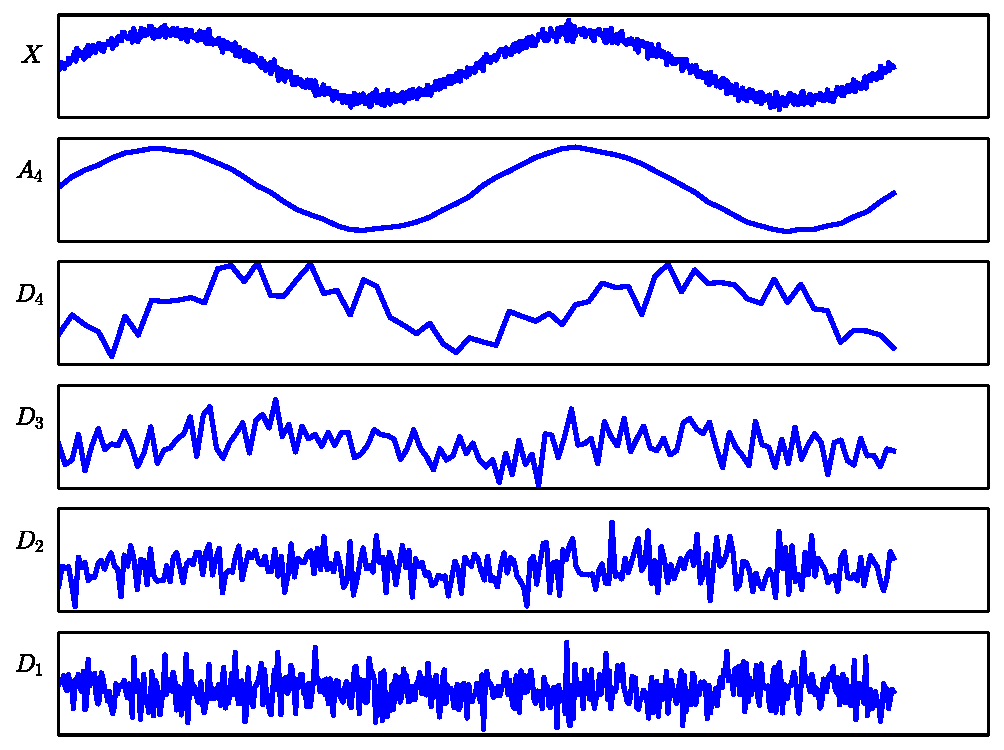
\includegraphics[width = 0.5\textwidth]{dwt1D}
\caption{A level 4 wavelet decomposition of a signal. The top panel is the original signal,
the next panel down is the approximation, and the remaining panels are the detail coefficients.
Notice how the approximation resembles a smoothed version of the original signal, while the
details capture the high-frequency oscillations and noise.}
\label{fig:dwt1D}
\end{figure}

In practice, we are often interested in analyzing discrete signals with compact support (that is,
finite-time signals that we have sampled at a finite number of points). If wavelet analysis is
to be of any use, we first need an efficient way to calculate the discrete wavelet transform.
The process described in the first section, while intuitive and illustrative of the mathematical
principles
behind wavelet analysis, is not the best approach to calculating the wavelet coefficients. It
turns out that the discrete wavelet transform can be implemented as an iterated low-pass/high-pass
filter bank, one iteration of which is shown graphically in the figure. We present the
algorithm without getting into the details of why it works.


The algorithm goes as follows.
Given an input matrix of size $2^n \times 2^n$, first operate on the rows as you would
in the one-dimensional Wavelet transform (i.e. convolve each row with the filters, then
downsample).
We then have two matrices of size $2^n \times 2^{n-1}$,
since each row has been downsampled by a factor of 2. Then for each of these two
intermediate matrices, operate on each column, yielding a total of four matrices of
size $2^{n-1} \times 2^{n-1}$. Figure \ref{fig:2dwt}
gives a graphical depiction of one iteration of the algorithm.

We initialize $LL_0$ to be the
original image matrix, and we terminate once the length of the rows or columns
is less than the length of the filters. We end up with a list of wavelet
coefficients, starting with the final approximation frame $LL_n$ followed by
collections of detail coefficients $(LH_n,HL_n,HH_n)$, $(LH_{n-1},HL_{n-1},HH_{n-1})$,
$\ldots$, $(LH_1,HL_1,HH_1)$. Note that at each iteration we operate first on the
rows (convolve with the filter, then downsample), and the we operate on the columns
of the resulting matrices (\emph{not} the original matrix). The size of the output
matrices have been reduced by a factor of two in both dimensions. As with the
one-dimensional algorithm, to reconstruct the image from the coefficients, we simply
reverse the process by upsampling, convolving, and adding (first the columns, then
the rows). We provide sample code for one iteration of the transform and the inverse.

\begin{lstlisting}
import numpy as np
from scipy.signal import fftconvolve

# given the current approximation frame image, and the filters lo_d and hi_d
# initialize empty arrays
temp = np.zeros([image.shape[0], image.shape[1]/2])
LL = np.zeros([image.shape[0]/2, image.shape[1]/2])
LH = np.zeros([image.shape[0]/2, image.shape[1]/2])
HL = np.zeros([image.shape[0]/2, image.shape[1]/2])
HH = np.zeros([image.shape[0]/2, image.shape[1]/2])

# low-pass filtering along the rows
for i in xrange(image.shape[0]):
	temp[i] = fftconvolve(image[i], lo_d, mode='full')[1::2]

# low and hi-pass filtering along the columns
for i in xrange(image.shape[1]/2):
	LL[:,i] = fftconvolve(temp[:,i],lo_d,mode='full')[1::2]
    LH[:,i] = fftconvolve(temp[:,i],hi_d,mode='full')[1::2]

# hi-pass filtering along the rows
for i in xrange(image.shape[0]):
	temp[i] = fftconvolve(image[i], hi_d, mode='full')[1::2]

# low and hi-pass filtering along the columns
for i in xrange(image.shape[1]/2):
	HL[:,i] = fftconvolve(temp[:,i],lo_d,mode='full')[1::2]
    HH[:,i] = fftconvolve(temp[:,i],hi_d,mode='full')[1::2]
\end{lstlisting}
At this point, the variables \li{LL, LH, HL, HH} contain the current level of wavelet coefficients.
You would then store \li{(LH, HL, HH)} in a list, and feed \li{LL} back into the same
block of code (with \li{LL} replacing \li{image}) to obtain the next level of coefficients.

Now, given a current level of wavelet coefficients, here is the code to recover the previous
approximation frame, which is the crucial step in the inverse transform.
\begin{lstlisting}
# given current coefficients LL, LH, HL, HH
# initialize temporary arrays
n = LL.shape[0]
temp1 = np.zeros([2*n,n])
temp2 = np.zeros([2*n,n])
up1 = np.zeros(2*n)
up2 = np.zeros(2*n)

# upsample and filter the columns of the coefficient arrays
for i in xrange(n):
	up1[1::2] = HH[:,i]
	up2[1::2] = HL[:,i]
	temp1[:,i] = fftconvolve(up1, hi_r)[1:] + fftconvolve(up2, lo_r)[1:]
	up1[1::2] = LH[:,i]
	up2[1::2] = LL[:,i]
	temp2[:,i] = fftconvolve(up1, hi_r)[1:] + fftconvolve(up2, lo_r)[1:]

# upsample and filter the rows, then add results together
result = sp.zeros([2*n,2*n])
for i in xrange(2*n):
	up1[1::2] = temp1[i]
	up2[1::2] = temp2[i]
	result[i] = fftconvolve(up1, hi_r)[1:] + fftconvolve(up2, lo_r)[1:]
\end{lstlisting}

\begin{problem}
Build off of the sample code to fully implement the two-dimensional discrete
wavelet transform as described above.
As before, the input to your function should consist of
three arrays: the input image, the low-pass filter, and the high-pass filter.
You should return a list of the following form: $$[LL_n,(LH_n,HL_n,HH_n), \ldots
,(LH_1,HL_1,HH_1)].$$

The inverse wavelet transform function should take as input a list
of that same form, as well as the reconstruction low-pass and high-pass filters,
and should return the reconstructed image.
\end{problem}
\end{comment}

\begin{comment}
This section could be cool, but it's not hashed out very well yet.
\section*{Edge Detection}
It is often useful to identify the edges of objects and figures
represented in images. The edge information can be used to classify images
and group them with other similar images (this is part of a field called
\textit{computer vision}), to segment the image into component parts, to
sharpen blurry images, to filter out unnecessary details of the image,
and so forth. Of course, our human eyes are very adept at recognizing edges,
but enabling a computer to do the same is much more difficult. An edge can
be thought of as a discontinuity in the image or a region of high contrast
in either color or brightness. We can therefore leverage the high-frequency
detail coefficients of the wavelet transform to detect the edges. Execute the
following code:
\begin{lstlisting}
>>> # calculate one level of wavelet coefficients
>>> coeffs = pywt.wavedec2(lena,'haar', level=1)
\end{lstlisting}

Note that the approximation coefficients are very close to the original
image, while the detail coefficients are much more sparse, and roughly
capture the edges in the image. In particular, the upper right coefficients
emphasize the vertical edges, the lower left coefficients emphasize the
horizontal edges, and the lower right coefficients emphasize the diagonal
edges.

\begin{problem}
Now zero out the approximation coefficients and use your inverse DWT
function to recreate the image. Plot its absolute value. This image is
a fairly good representation of the edges. If we add this to the original
image, we can increase the contrast at the edges (that is, make the dark
side darker, and the light side lighter). Do this, and plot the original
image side-by-side with the sharpened image. What do you notice? There
are many image-sharpening techniques, and those based on wavelets
are more sophisticated than what we have done here, but this gives the
basic idea.
\end{problem}
the above section needs work, or maybe should be taken out completely.
\end{comment}

\begin{comment}
This section is good, but there's just not room for it in this lab if we
want a fairly complete section on image compression.
\section*{Noise Removal}
Noise in an image can be defined as unwanted visual artifacts that
obscure the true image. Images can acquire noise from a variety of
sources, including the camera, transmission, and image processing
algorithms. Noise can be completely random and incoherent (as in
Figure \ref{fig:incoherent}), or it can be coherent and display
visual patterns (Figure \ref{fig:coherent}). In this section, we will
focus on reducing a particular type of random noise in images, called
\textit{Gaussian white noise}.

\begin{figure}[t]
\minipage{0.49\textwidth}
    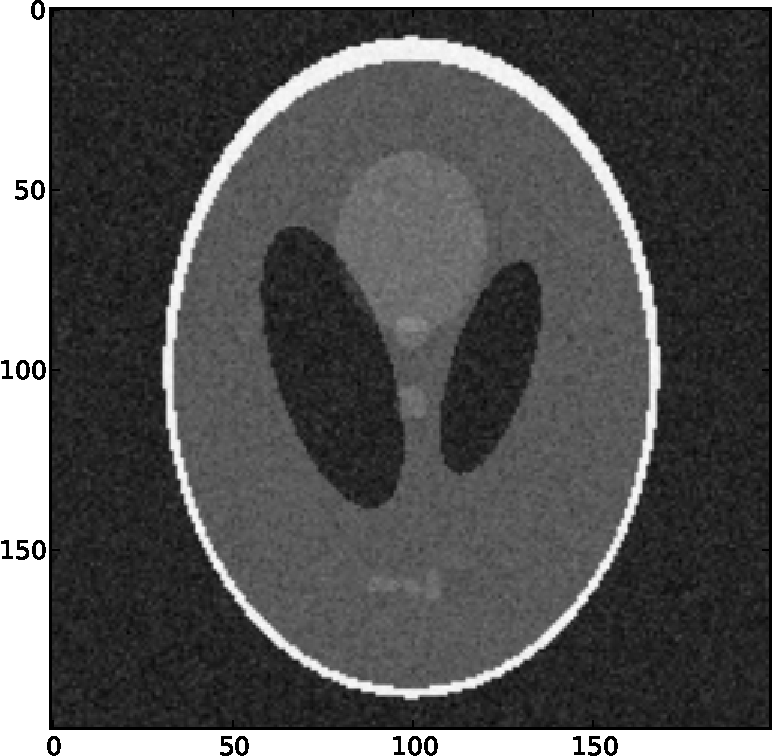
\includegraphics[width=\linewidth]{phantom_random.pdf}
    \caption{The Phantom image with incoherent noise}
    \label{fig:incoherent}
\endminipage\hfill
\minipage{0.49\textwidth}
    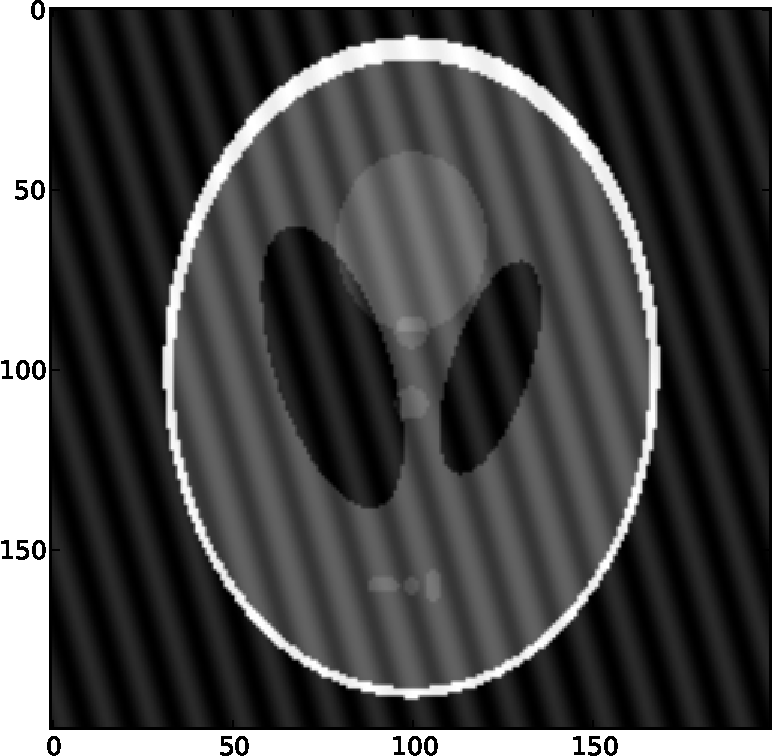
\includegraphics[width=\linewidth]{phantom_coherent.pdf}
    \caption{The Phantom image with coherent noise}
    \label{fig:coherent}
\endminipage
\end{figure}

An image that is distorted by Gaussian white noise is one in which
every pixel has been perturbed by a small amount, such that the
perturbations are normally distributed. We can easily add such noise
to an image using the \li{np.random.normal} function.

\begin{lstlisting}
>>> noisyLena = lena + np.random.normal(scale=20, size=lena.shape)
>>> plt.imshow(noisyLena, cmap=plt.cm.Greys_r)
>>> plt.show()
\end{lstlisting}

Given an image with Gaussian white noise, how do we go about reducing
the noise level? Our approach will be based on the idea of thresholding.
It turns out that images are often sparse in the wavelet basis,
particularly in the high-frequency details. The Gaussian noise, however,
is very high frequency, and thus its wavelet transform will be
concentrated in high-frequency wavelet coefficients (of magnitude
roughly proportional to the variance of the noise). We can therefore
reduce the noise while preserving the true image by shrinking the
detail coefficients via hard or soft thresholding.

Given a positive threshold value $\tau$, hard thresholding sets
every wavelet coefficient whose magnitude is less than $\tau$ to
zero, while leaving the remaining coefficients untouched. Soft
thresholding also zeros out all coefficients of magnitude less than
$\tau$, but in addition maps every other coefficient $\beta$ to
$\beta - \tau$ if $\beta > 0$ or $\beta + \tau$ if $\beta < 0$.

Implementing these simple thresholding algorithms in Python is
straight-forward, but PyWavelets already provides this functionality.
The following code gives an example.

\begin{lstlisting}
>>> A = np.arange(-4,5).reshape(3,3)
>>> A
array([[-4, -3, -2],
       [-1,  0,  1],
       [ 2,  3,  4]])
>>> pywt.thresholding.hard(A,1.5)
array([[-4, -3, -2],
       [ 0,  0,  0],
       [ 2,  3,  4]])
>>> pywt.thresholding.soft(A,1.5)
array([[-2.5, -1.5, -0.5],
       [ 0. ,  0. ,  0. ],
       [ 0.5,  1.5,  2.5]])
\end{lstlisting}

Once the coefficients have been thresholded, we take the inverse
wavelet transform to recover the denoised image. This can be done
by calling the \li{waverec2} function, providing the list of Wavelet
coefficients as well as the name of the desired Wavelet as arguments.
The threshold value is generally a function of the variance of the noise,
and in real situations, we do not know what this variance is. In fact,
noise variance estimation in images is a research area in its own
right, but this goes beyond the scope of this lab, and so we will
assume that we already have a decent estimate of the variance.

\begin{figure}[t]
    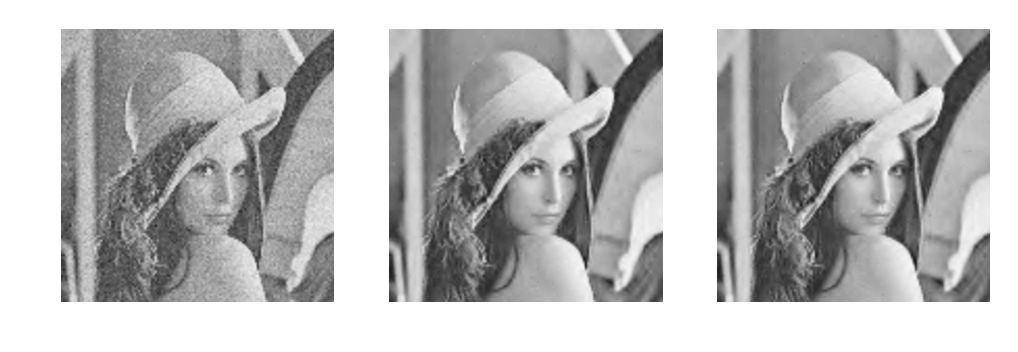
\includegraphics[width=\linewidth]{denoise.pdf}
    \caption{Noisy Lena (left), denoised using hard thresholding (center),
    and denoised using soft thresholding (right).}
    \label{fig:denoise}
\end{figure}

\begin{problem}
Write functions that implement the hard and soft thresholding
techniques. The inputs should be a list of wavelet coefficients
in the usual form, as well as the threshold value. The output
should be the thresholded wavelet coefficients (also in
the usual form). Remember that we only want to threshold the
detail coefficients, and not the approximation coefficients.
You should therefore leave the first entry of the input
coefficient list unchanged.
\end{problem}

\begin{problem}
Create a noisy version of the Lena image by adding Gaussian
white noise of mean 0 and standard deviation $\sigma = 20$ (i.e. \li{scale=20}).
Compute four levels of the wavelet coefficients using the Daubechies 4 Wavelet,
and input these into your
thresholding functions (with $\tau = 3\sigma$ for the hard threshold,
and $\tau = 3\sigma/2$ for the soft threshold). Reconstruct the
two denoised images, and then plot these together alongside the
noisy image. Your output should match Figure \ref{fig:denoise}.

What do you notice? How does lowering or raising the
threshold affect the reconstructed images? What happens if you use
a different Wavelet?
\end{problem}
\end{comment}
